\cleardoublepage
\chapter{Game Play images}

This appendix shows game play captures. It goes through the three different game modes and shows how the gamer interacts with them using the physical instrument pieces.

\cleardoublepage

\section{Playing game mode}

\begin{figure}[ht!]
  \centering
  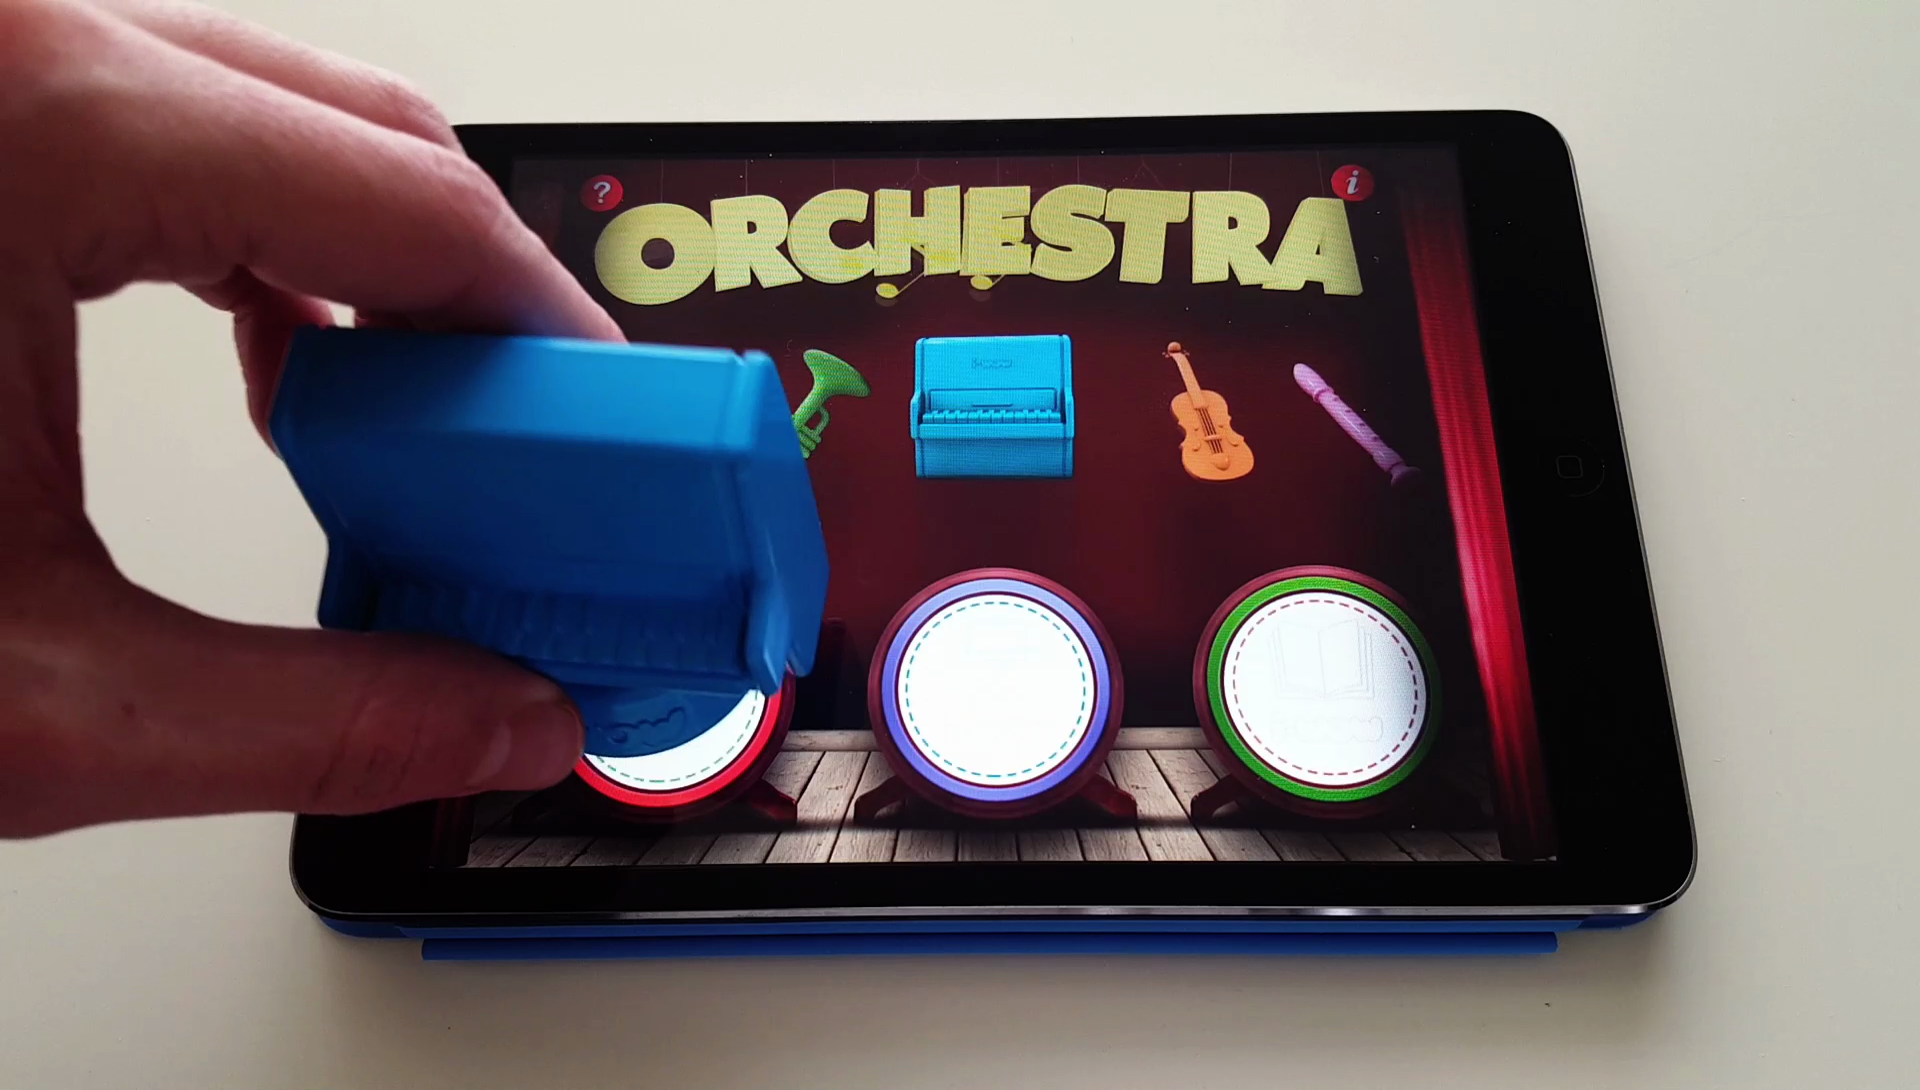
\includegraphics[width=350pt]{graphics/game-play/enter_playing_mode.png}
  \vspace{0.05cm}
  \caption{Entering playing game mode from home screen}
  \vspace{1cm}

  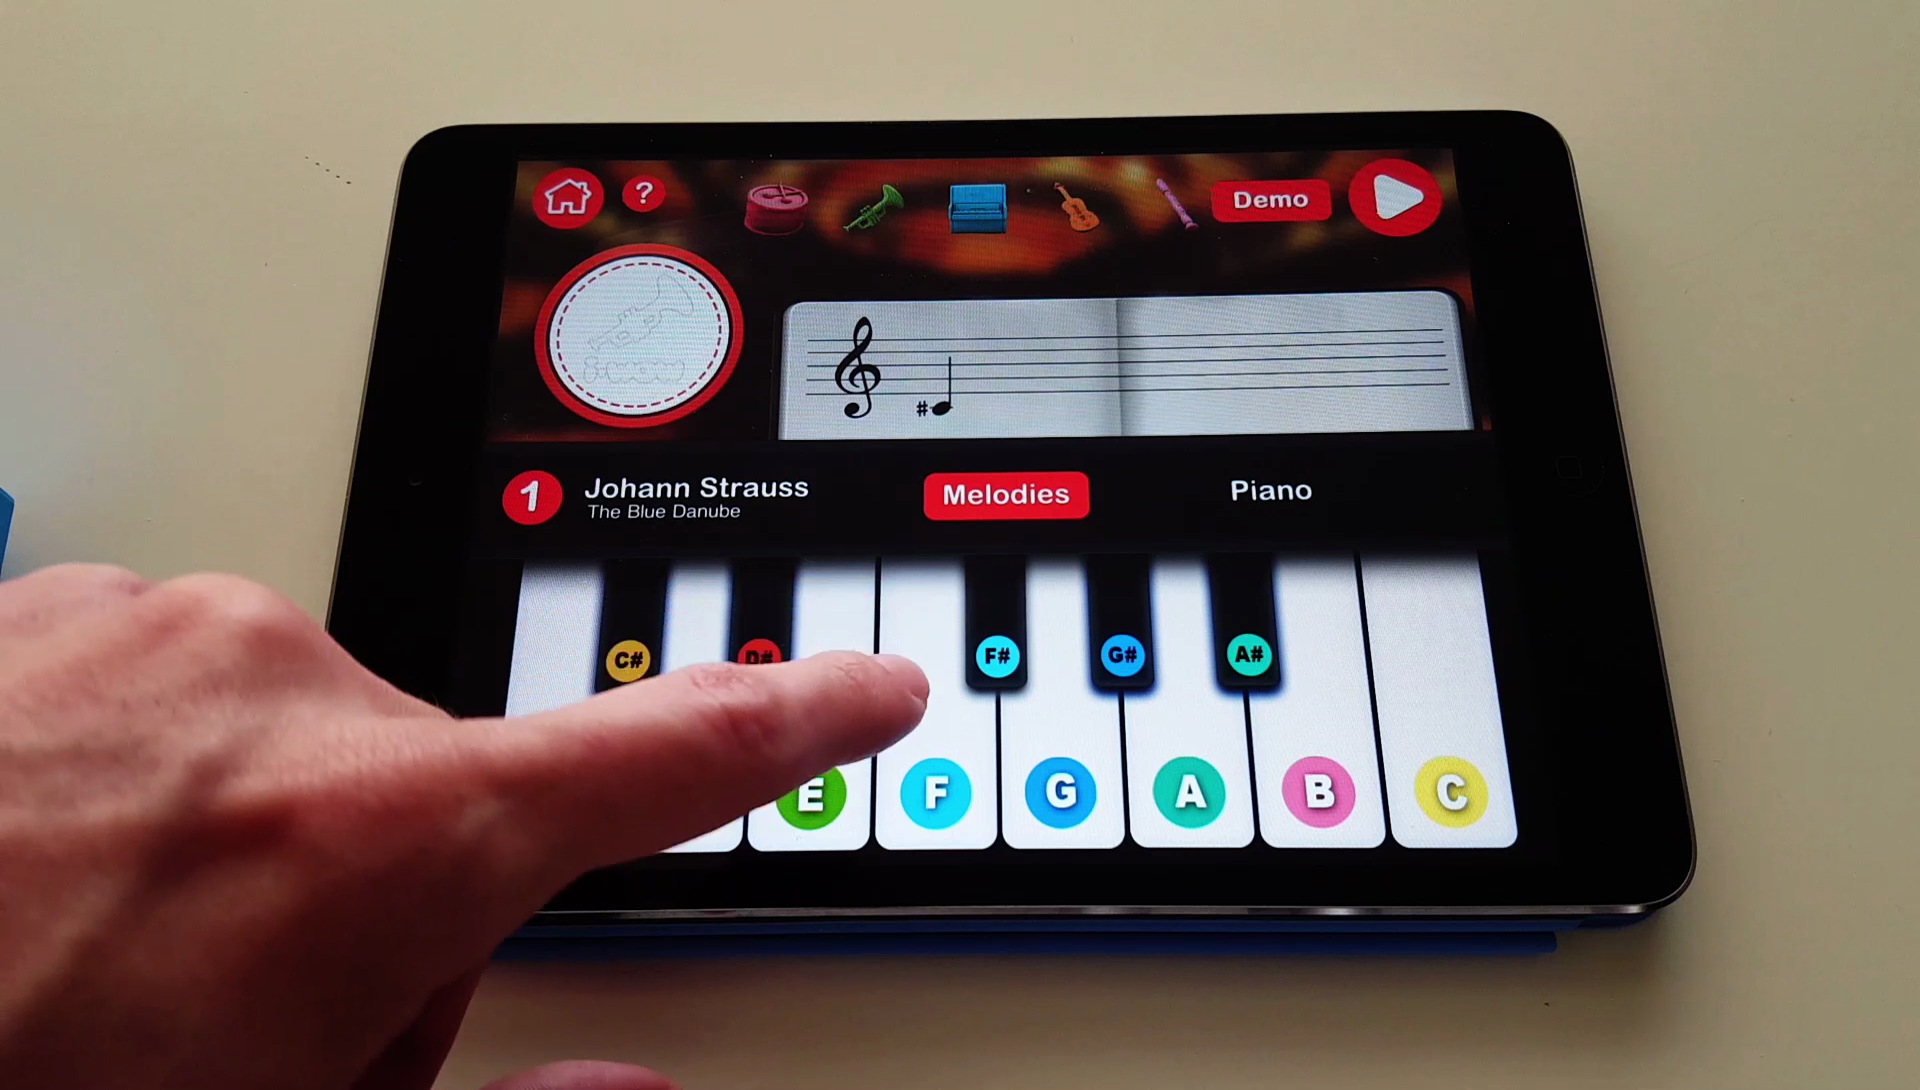
\includegraphics[width=350pt]{graphics/game-play/playing_piano_free.png}
  \vspace{0.05cm}
  \caption{Playing piano free mode}
\end{figure}

\begin{figure}[ht!]
  \centering
  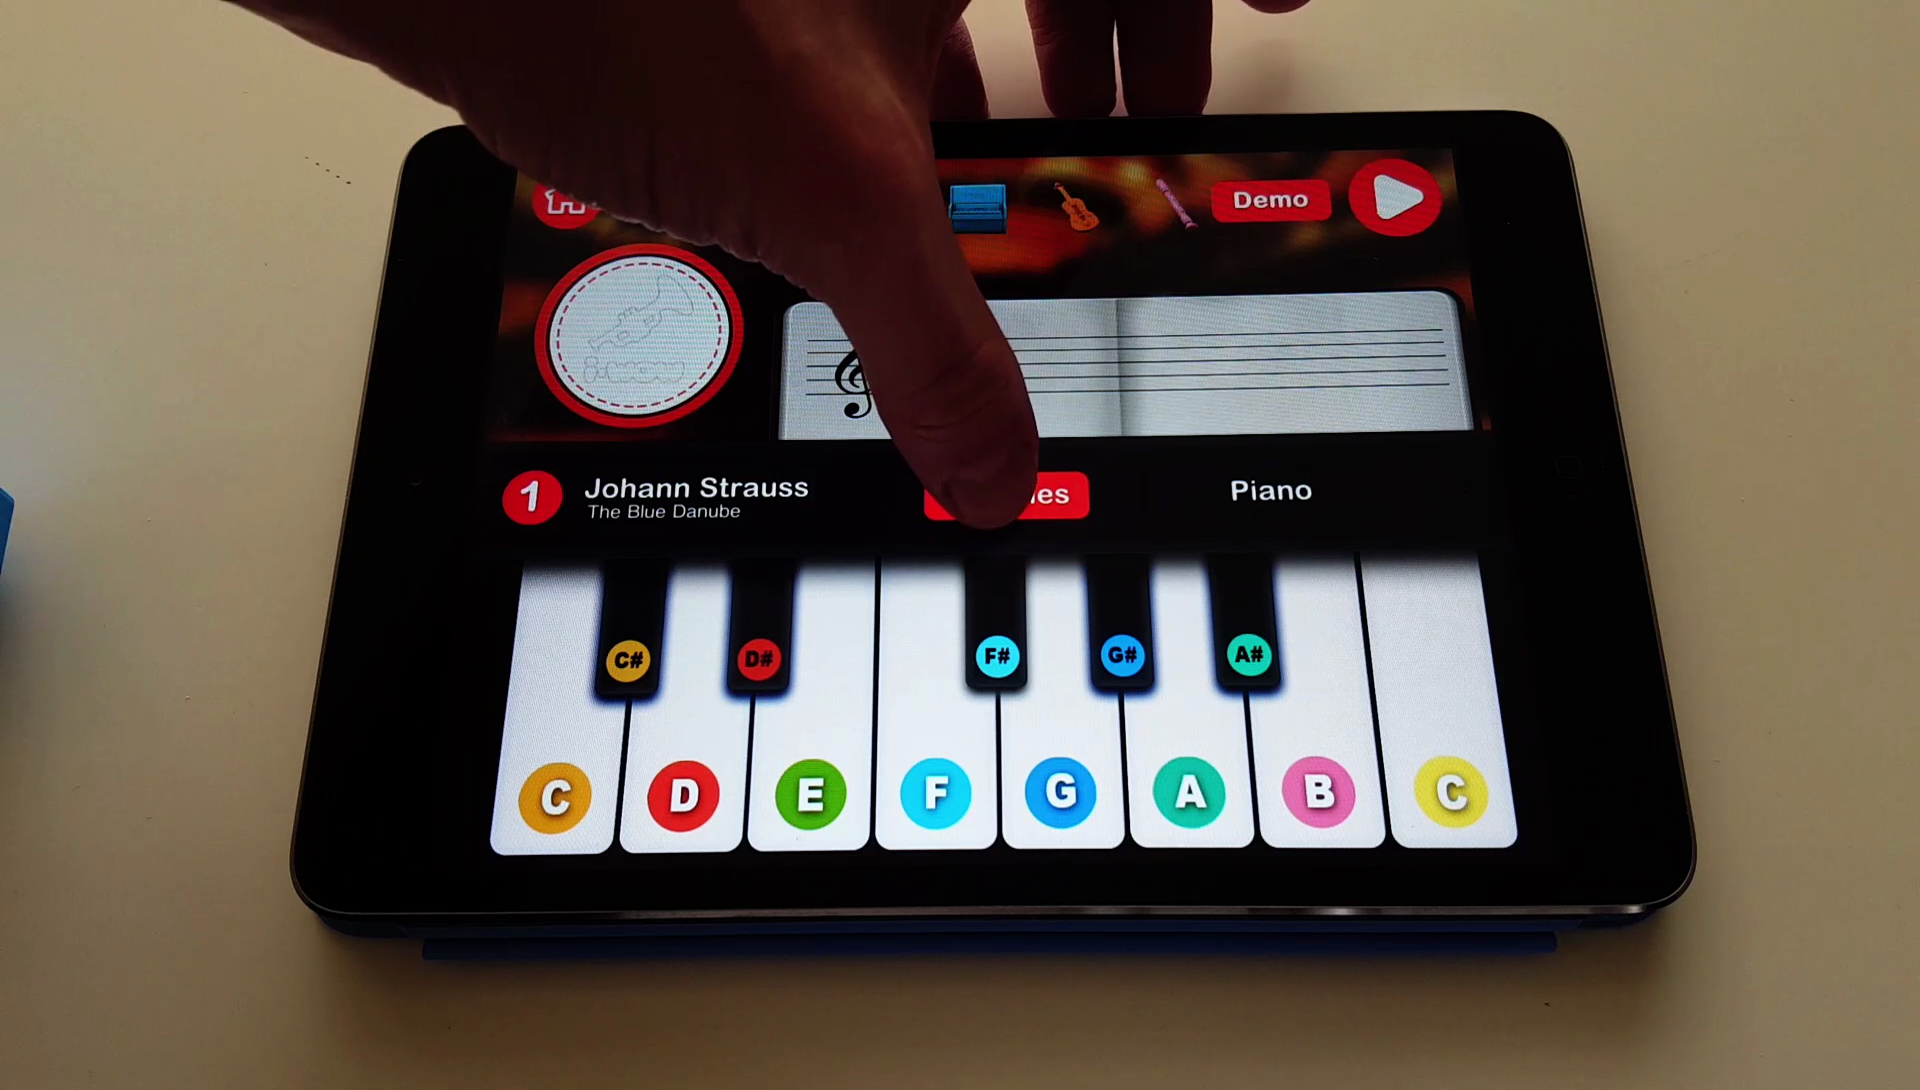
\includegraphics[width=350pt]{graphics/game-play/choose_melody_playing.png}
  \vspace{0.05cm}
  \caption{Opening melodies menu in playing game mode}
  \vspace{1cm}

  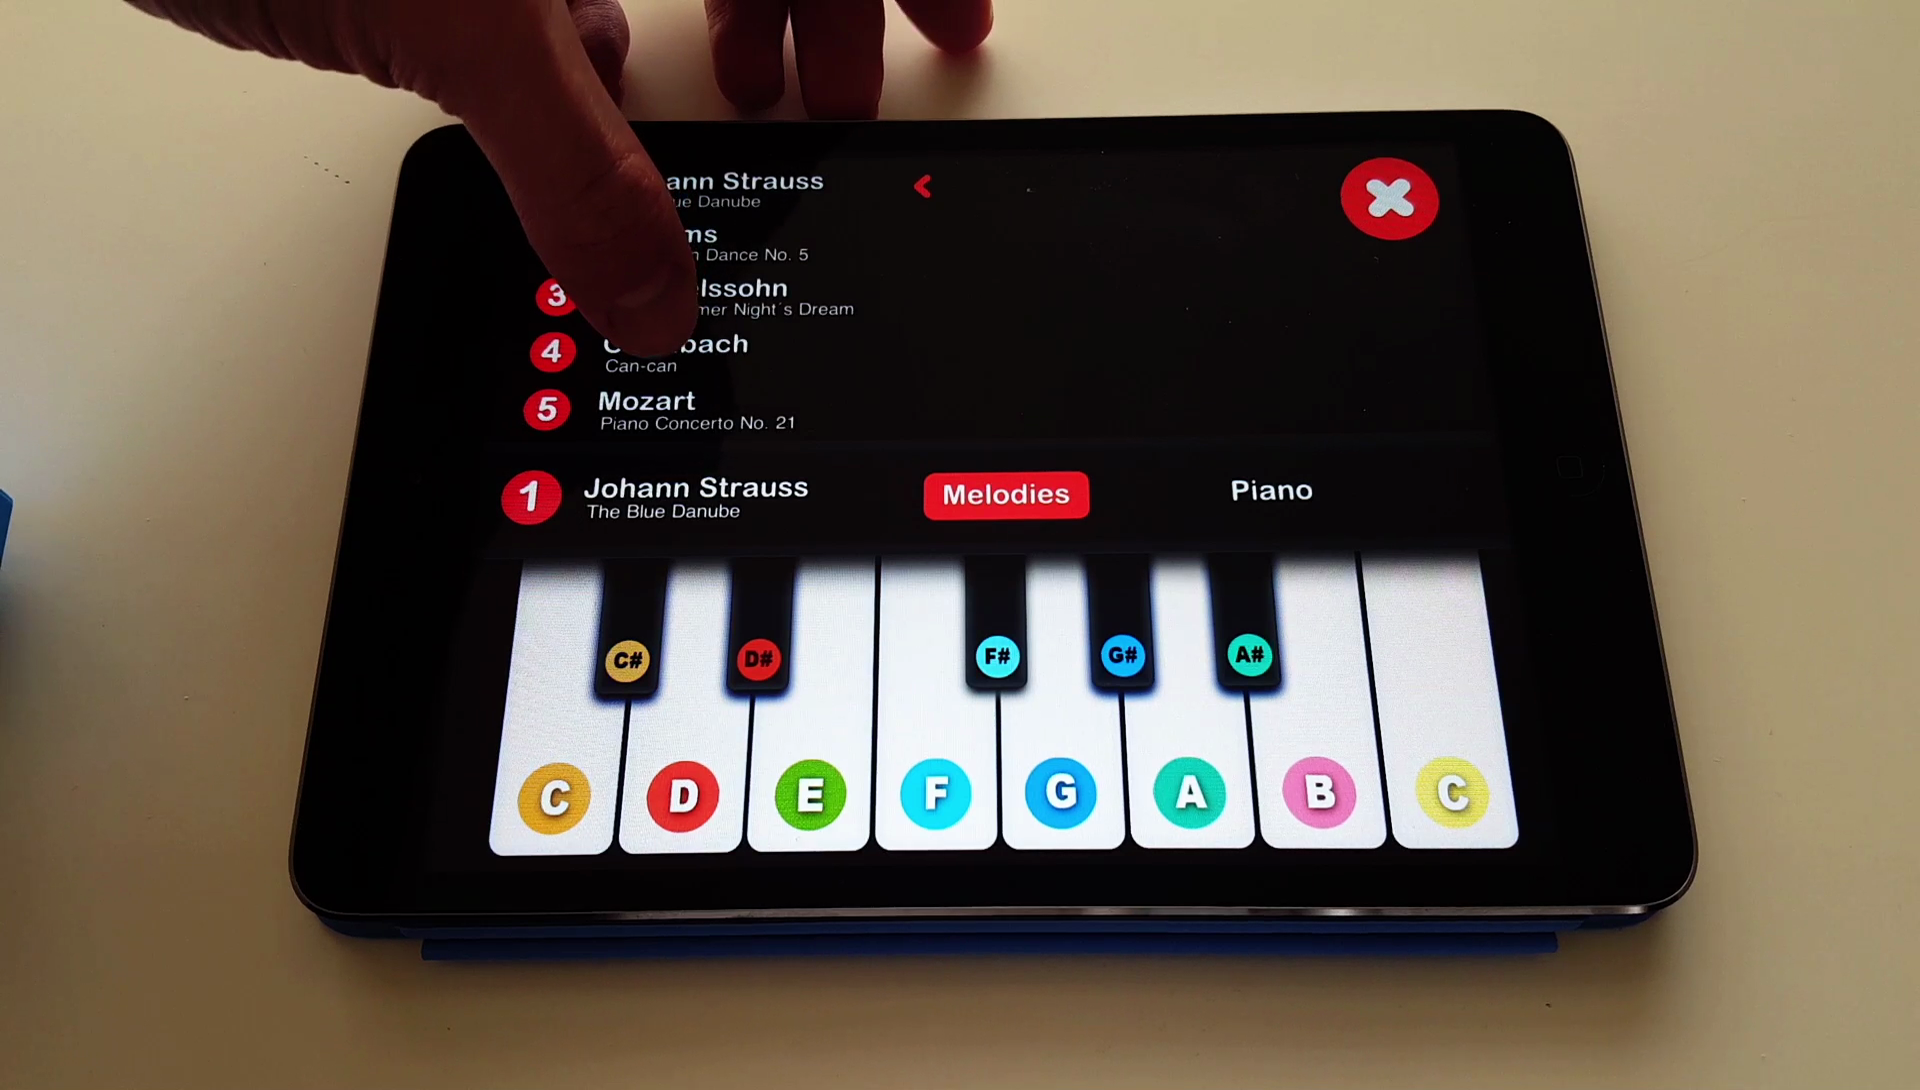
\includegraphics[width=350pt]{graphics/game-play/change_melody_playing.png}
  \vspace{0.05cm}
  \caption{Changing melody to be played in playing game mode}
\end{figure}

\begin{figure}[ht!]
  \centering
  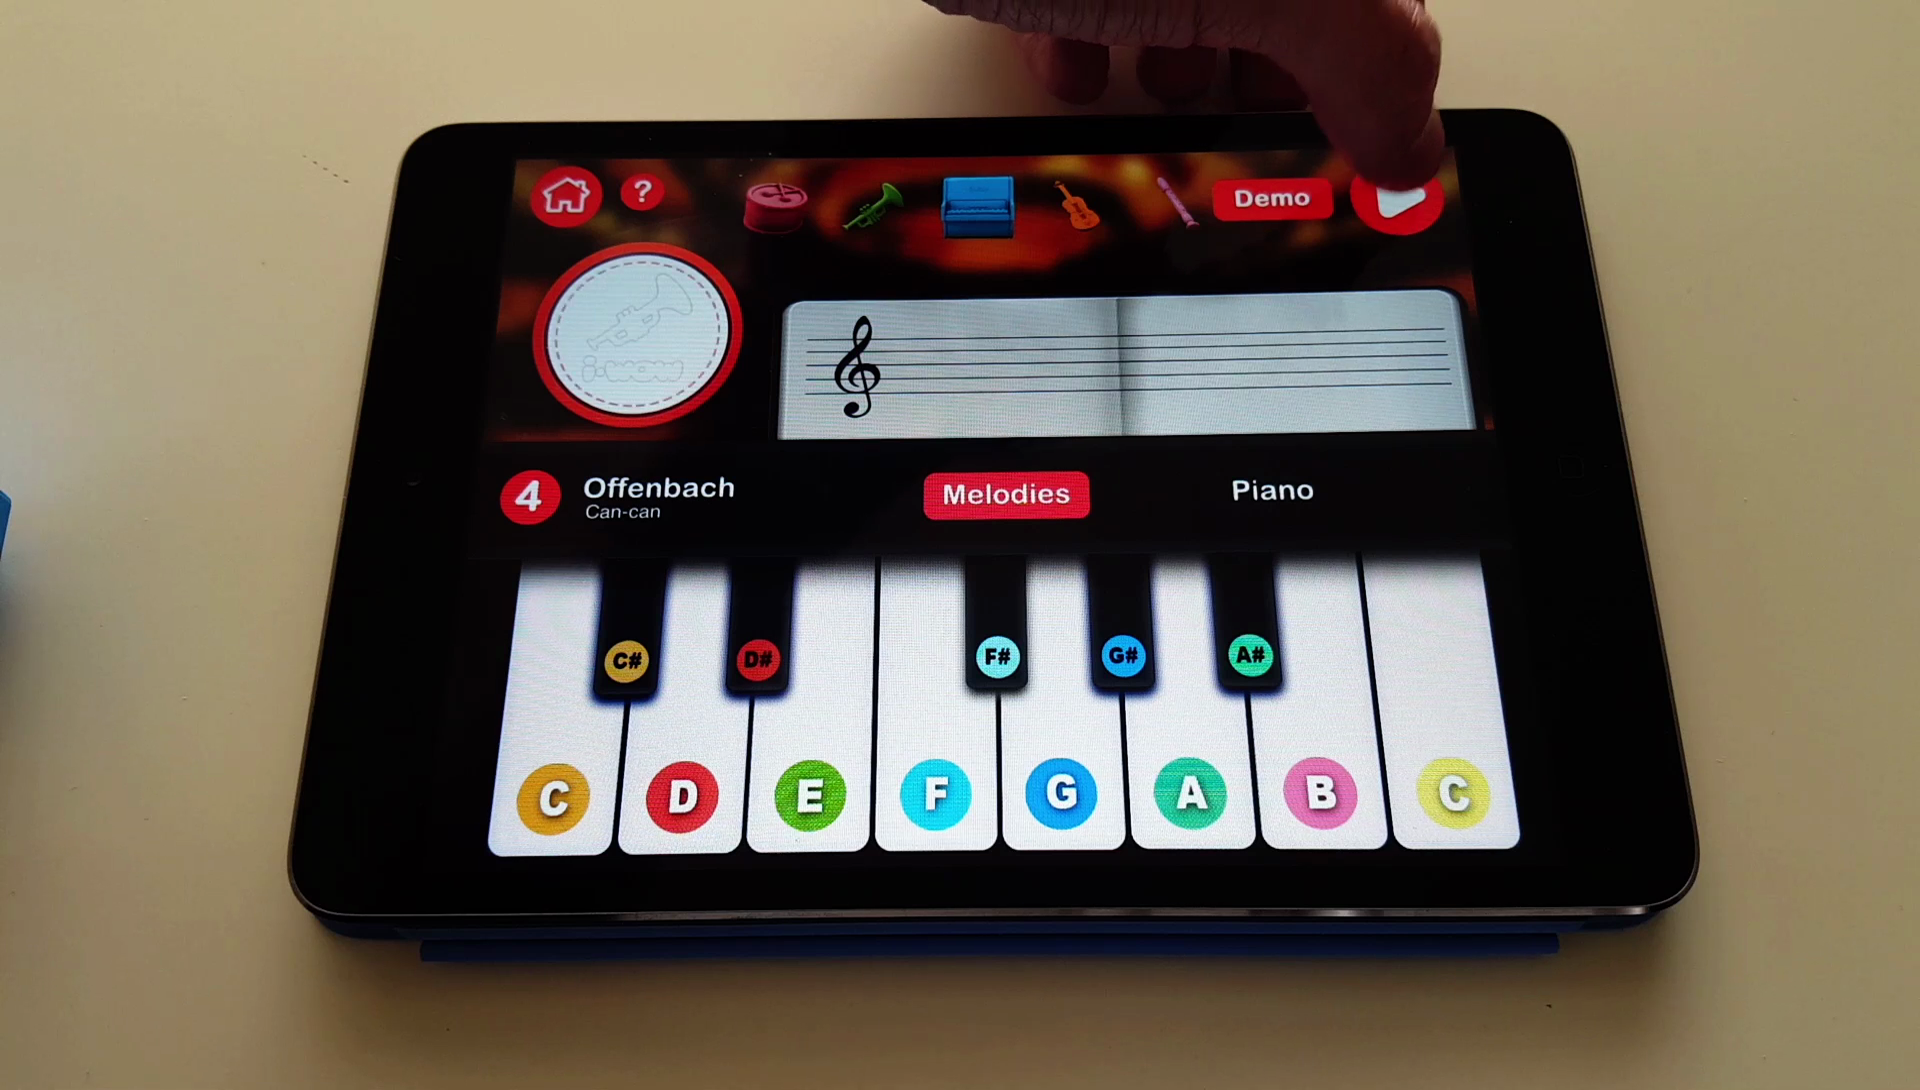
\includegraphics[width=350pt]{graphics/game-play/select_guided_mode.png}
  \vspace{0.05cm}
  \caption{Starting guided playing mode}
  \vspace{1cm}

  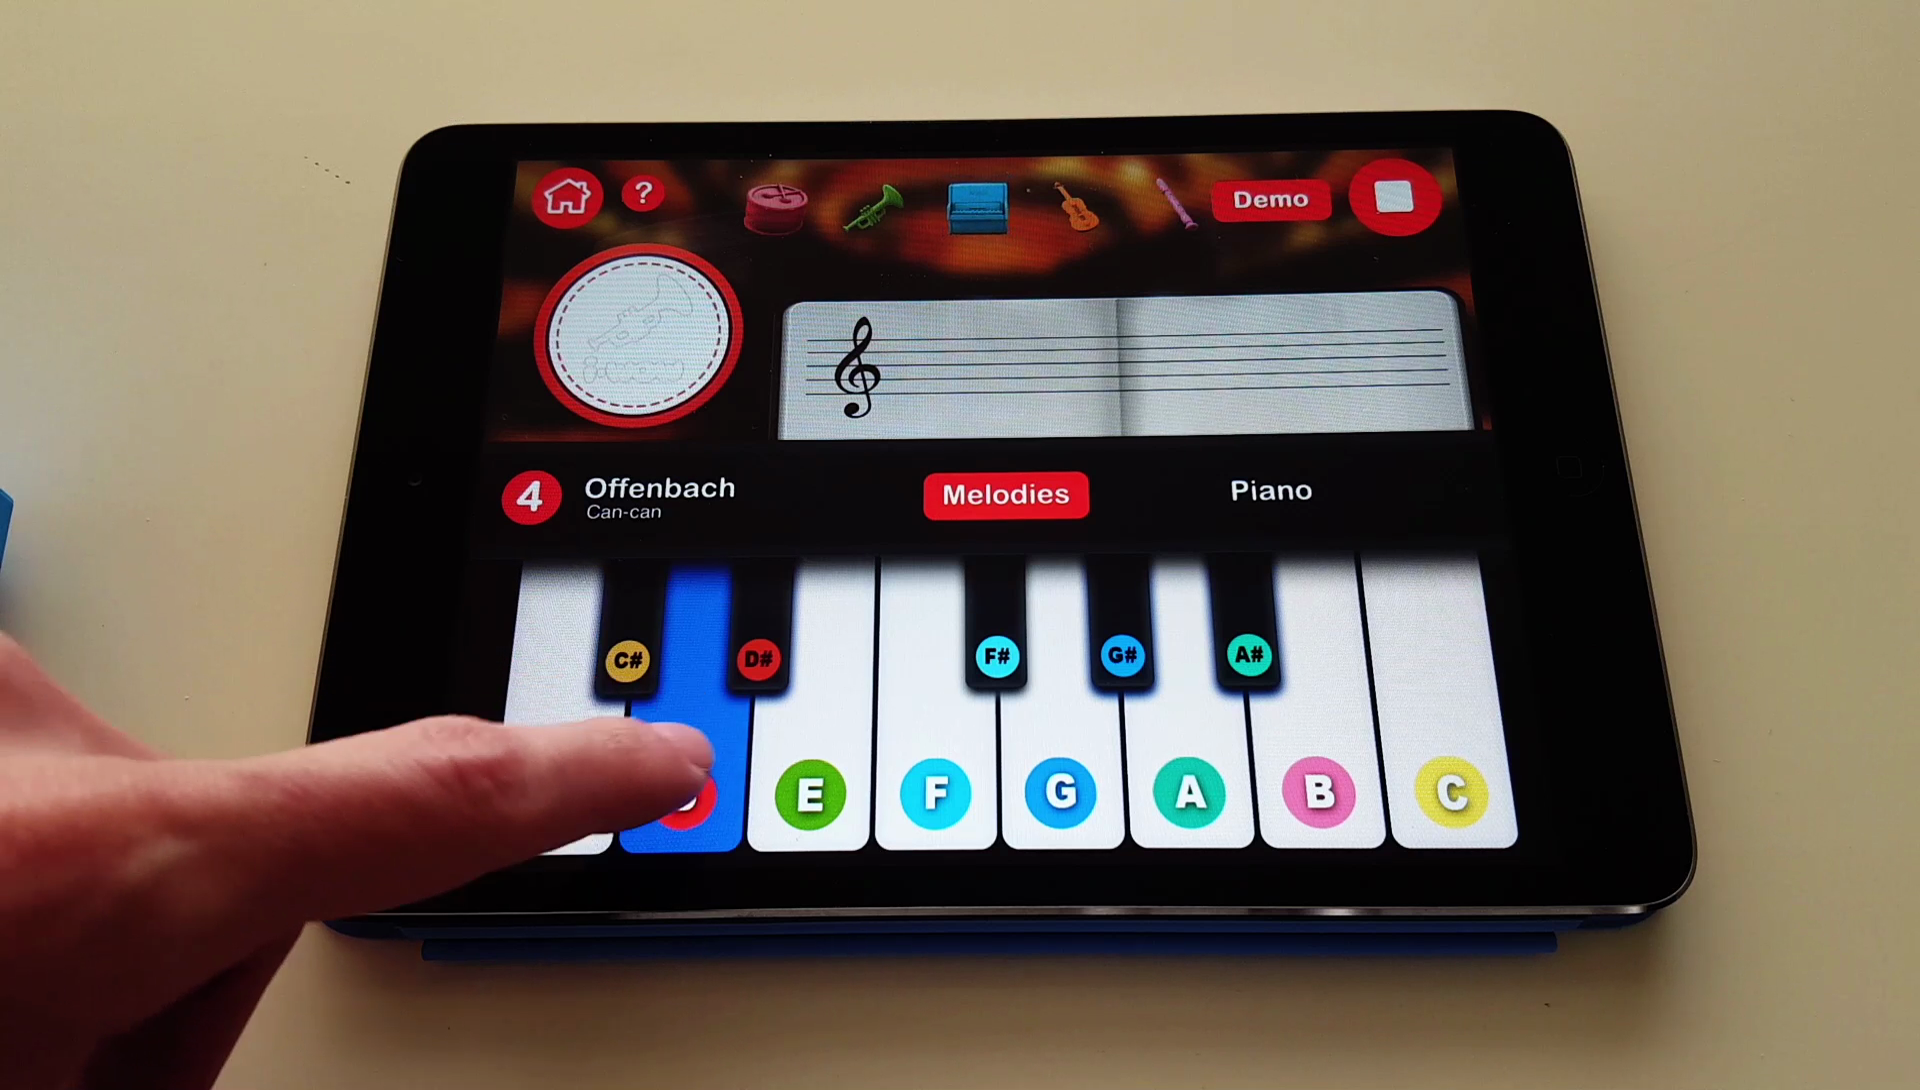
\includegraphics[width=350pt]{graphics/game-play/playing_piano_guided.png}
  \vspace{0.05cm}
  \caption{Playing piano guided}
\end{figure}

\begin{figure}[ht!]
  \centering
  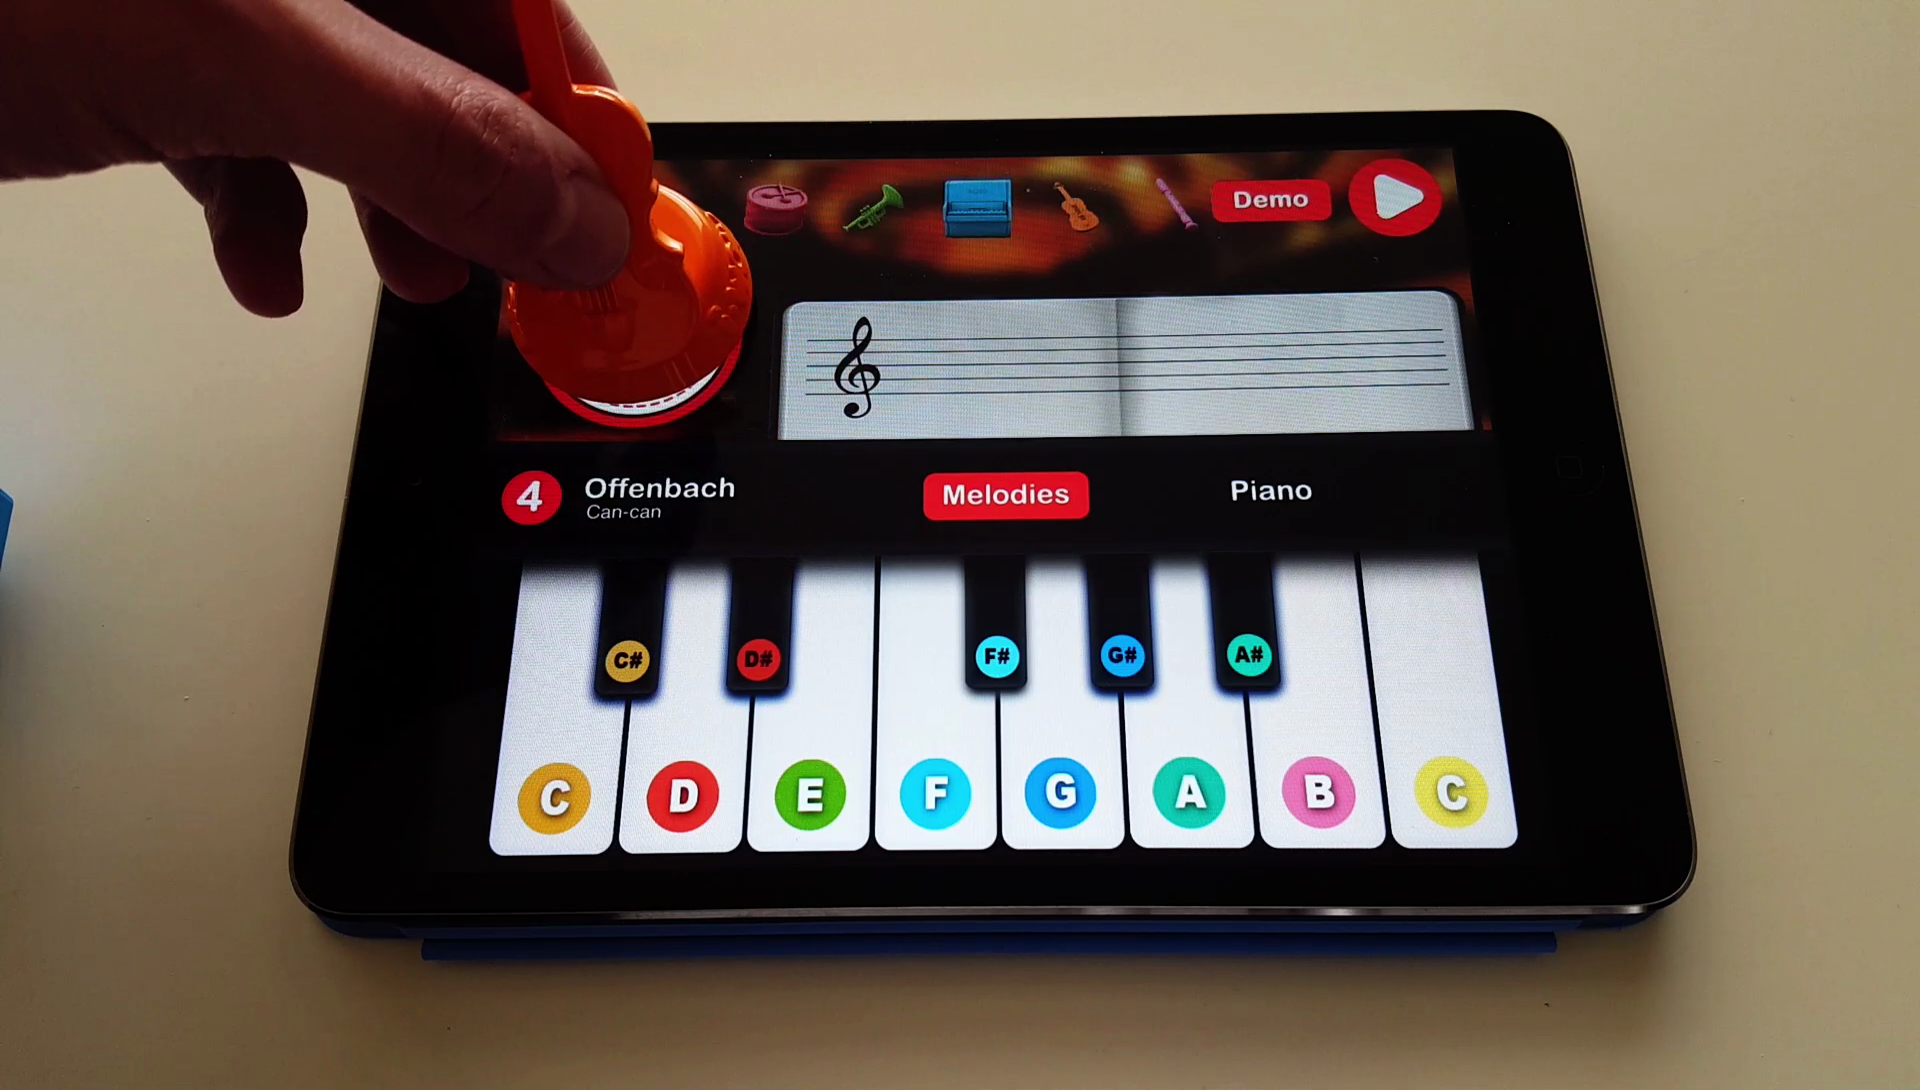
\includegraphics[width=350pt]{graphics/game-play/change_strings_playing.png}
  \vspace{0.05cm}
  \caption{Placing strings piece in playing game mode}
  \vspace{1cm}

  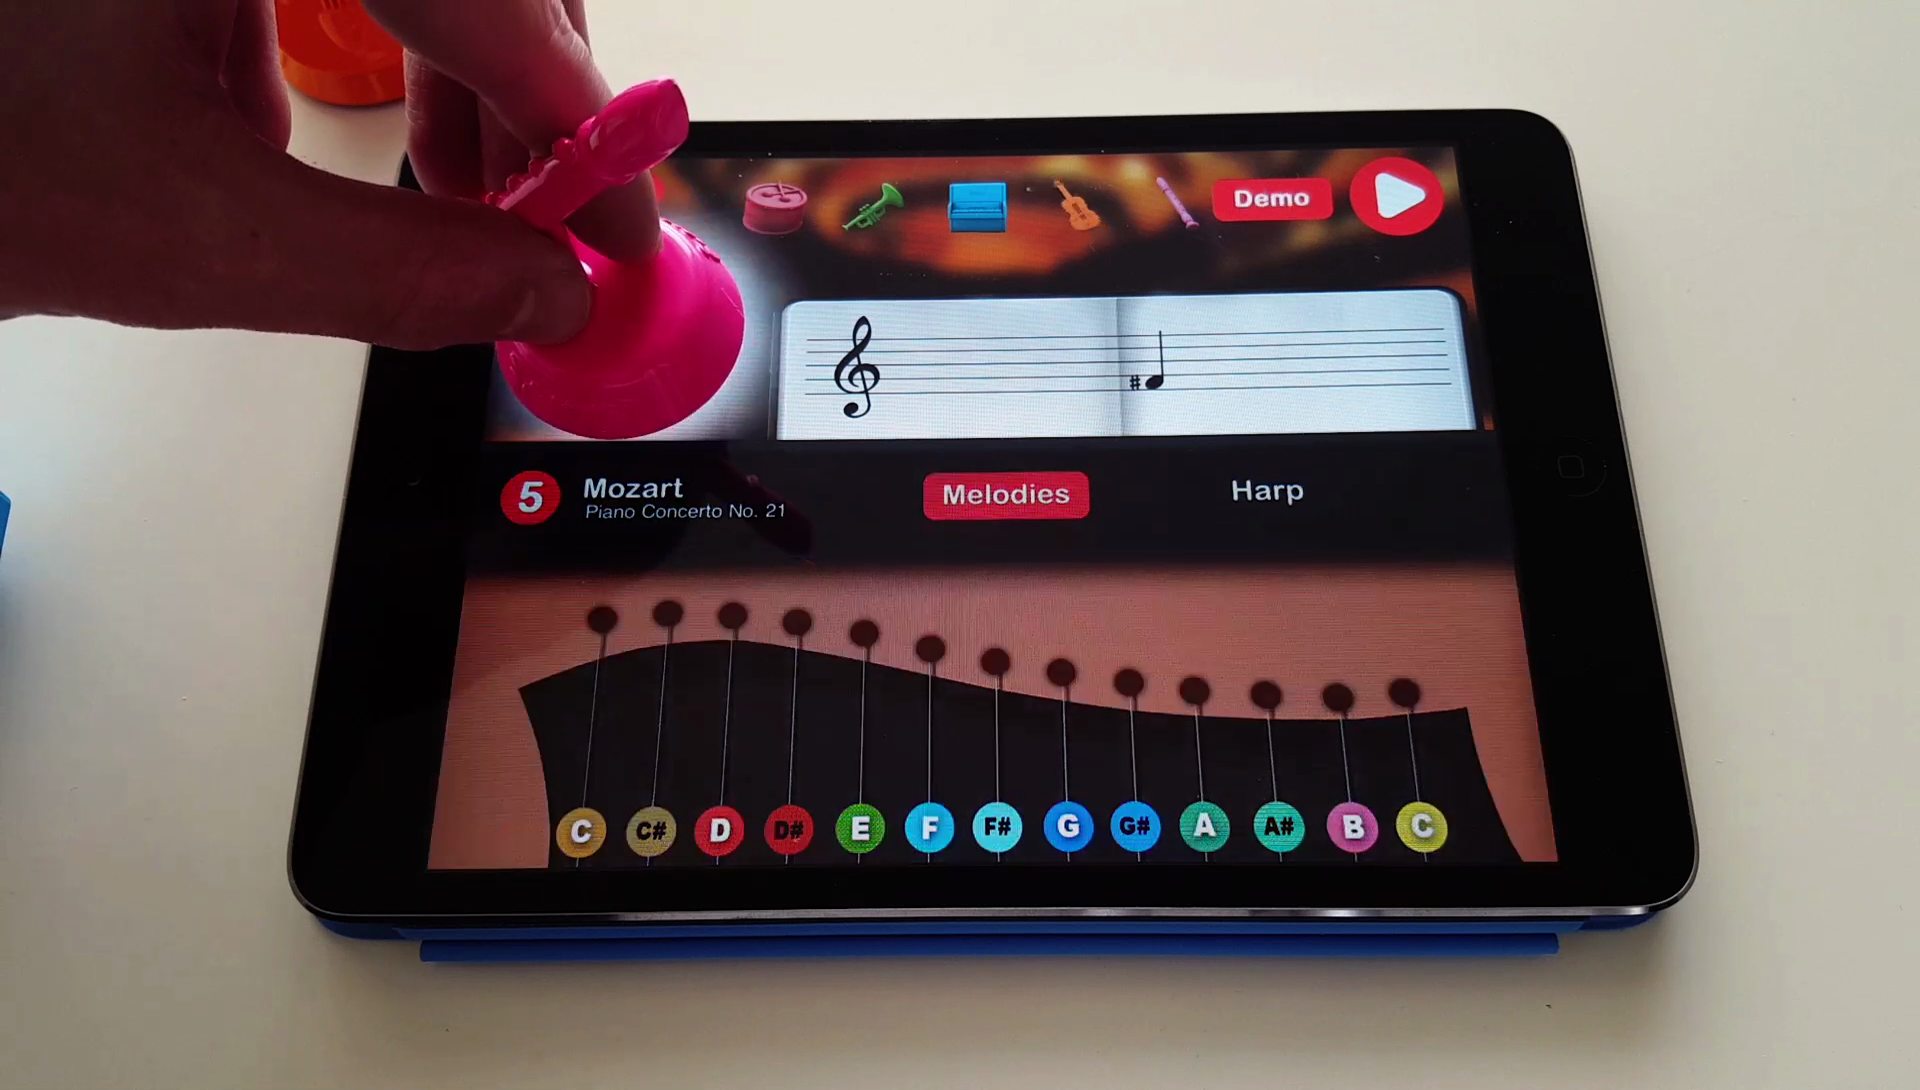
\includegraphics[width=350pt]{graphics/game-play/change_woodwind_playing.png}
  \vspace{0.05cm}
  \caption{Placing woodwind piece in playing game mode}
\end{figure}

\begin{figure}[ht!]
  \centering
  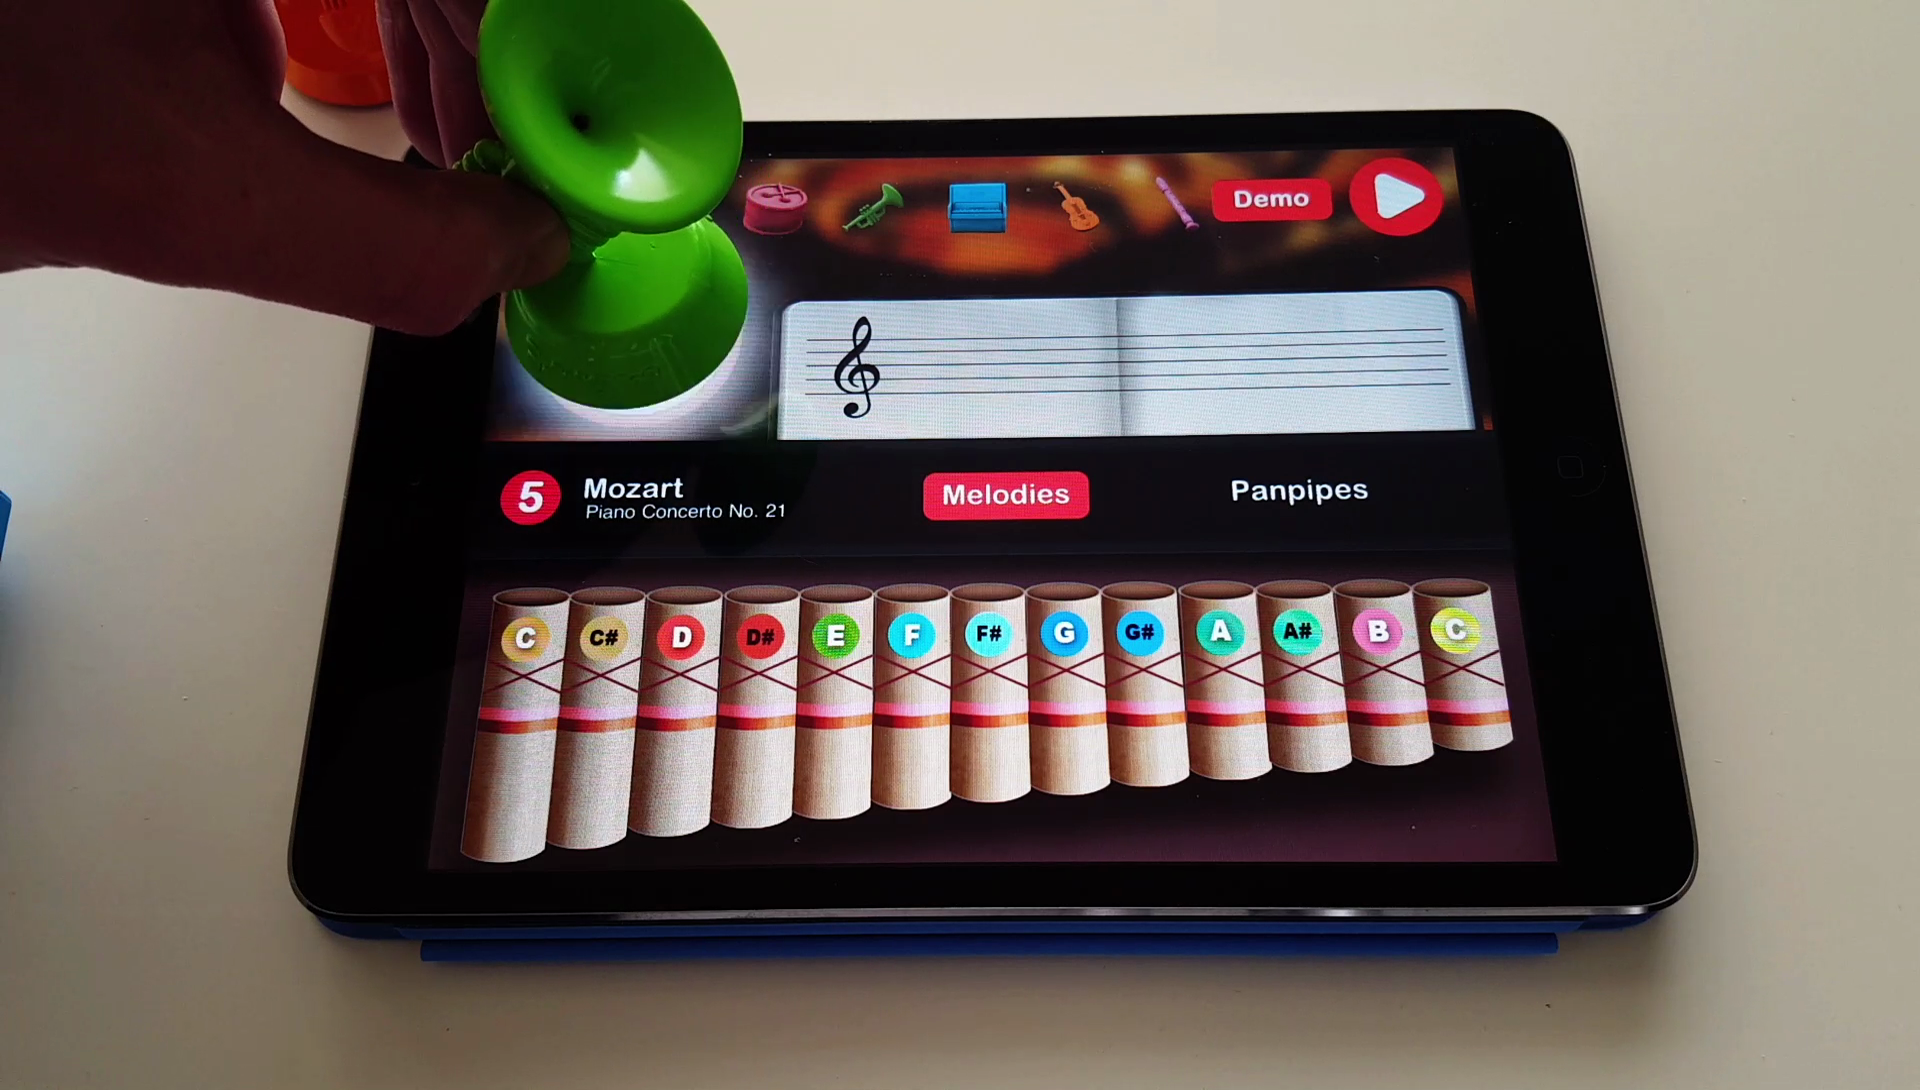
\includegraphics[width=350pt]{graphics/game-play/change_brass_playing.png}
  \vspace{0.05cm}
  \caption{Placing brass piece in playing game mode}
  \vspace{1cm}

  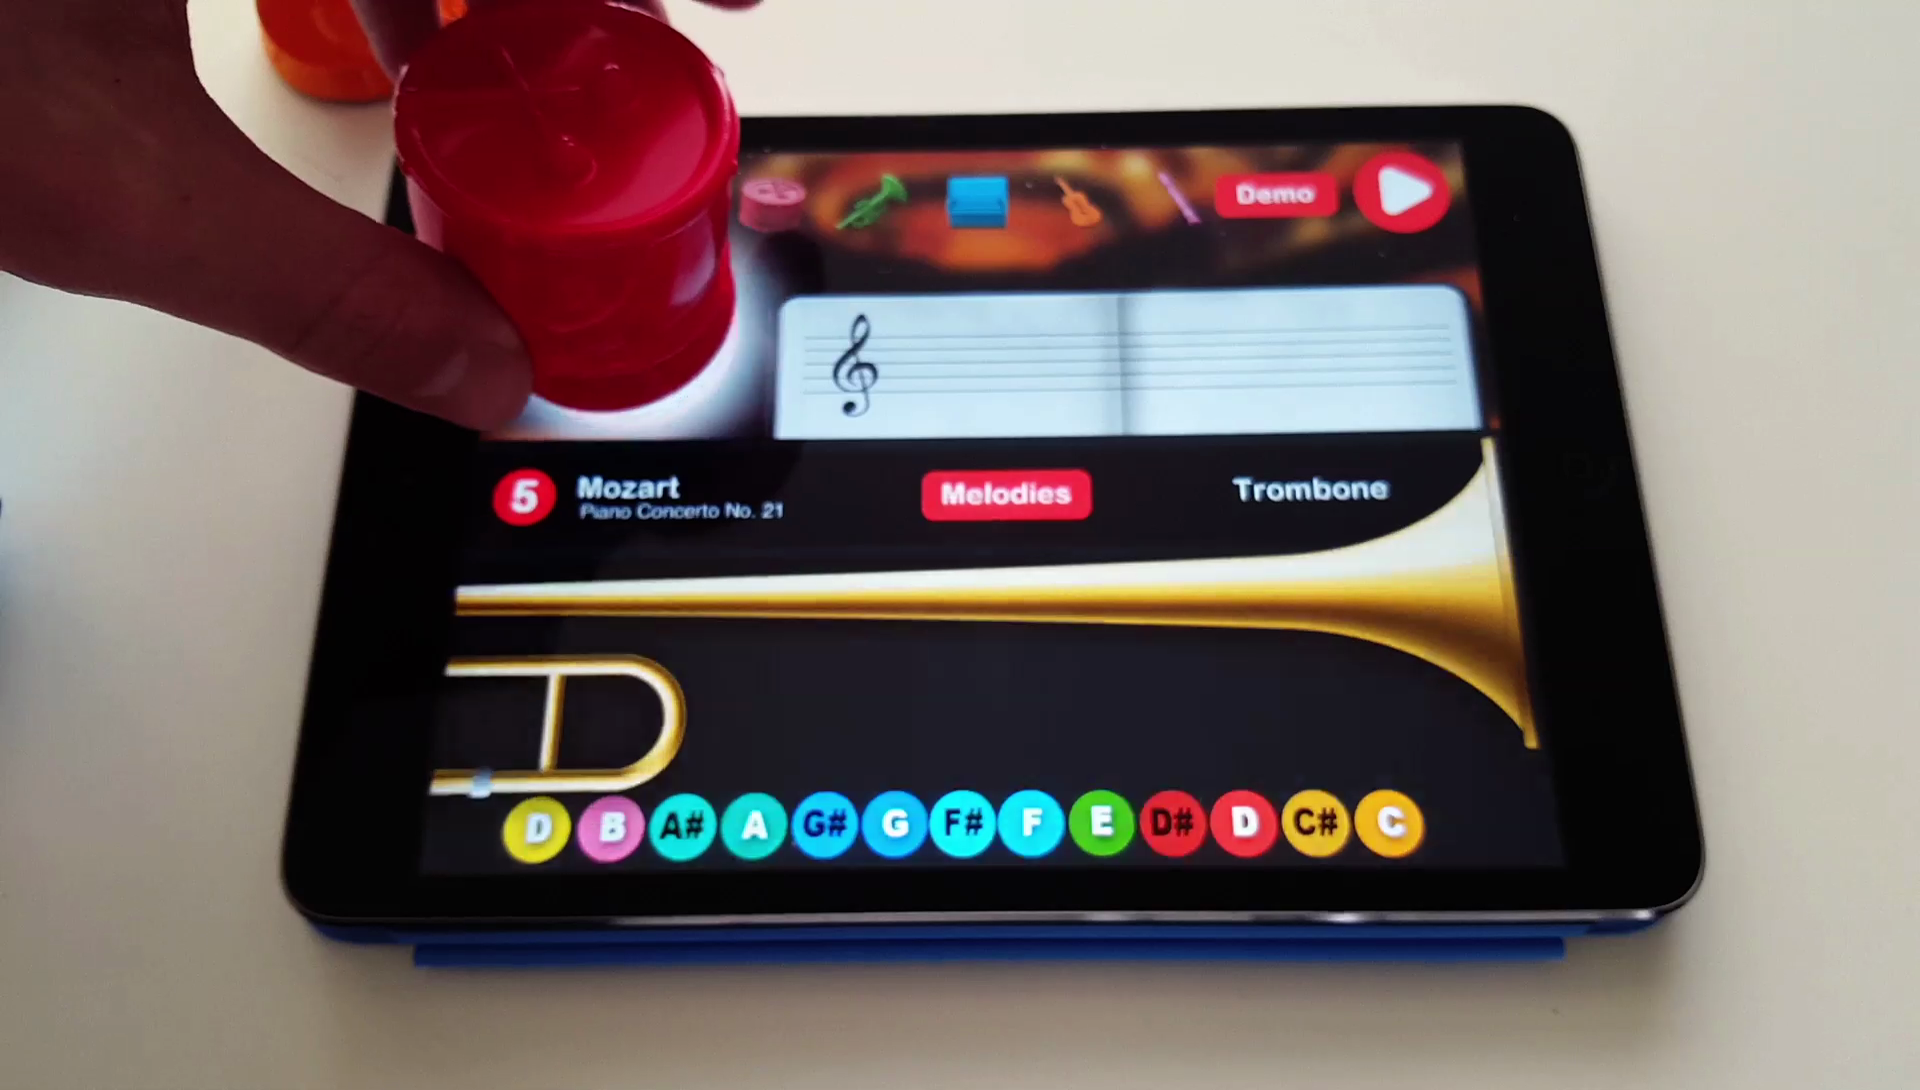
\includegraphics[width=350pt]{graphics/game-play/change_percussion_playing.png}
  \vspace{0.05cm}
  \caption{Placing percussion piece in playing game mode}
\end{figure}

\section{Conducting game mode}

\begin{figure}[ht!]
  \centering
  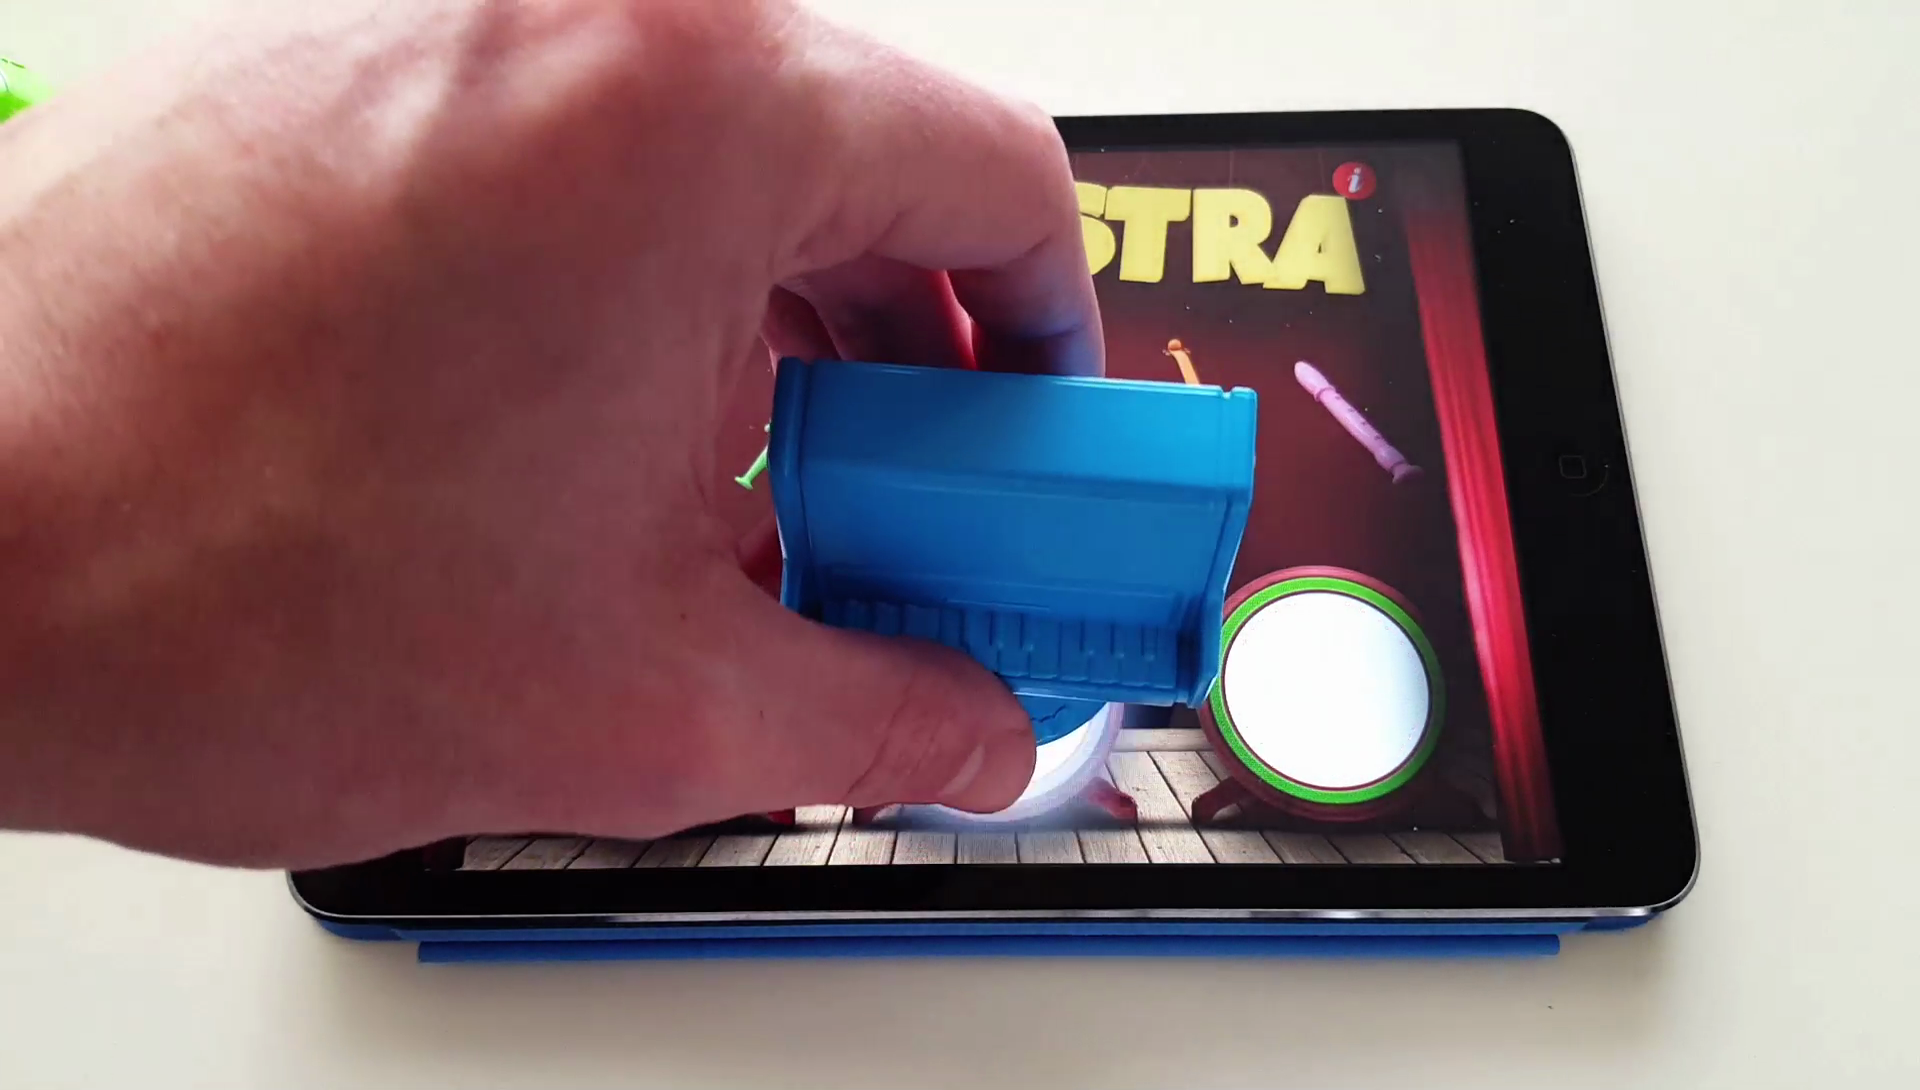
\includegraphics[width=350pt]{graphics/game-play/enter_conducting_mode.png}
  \vspace{0.05cm}
  \caption{Entering conducting game mode from home screen}
  \vspace{1cm}

  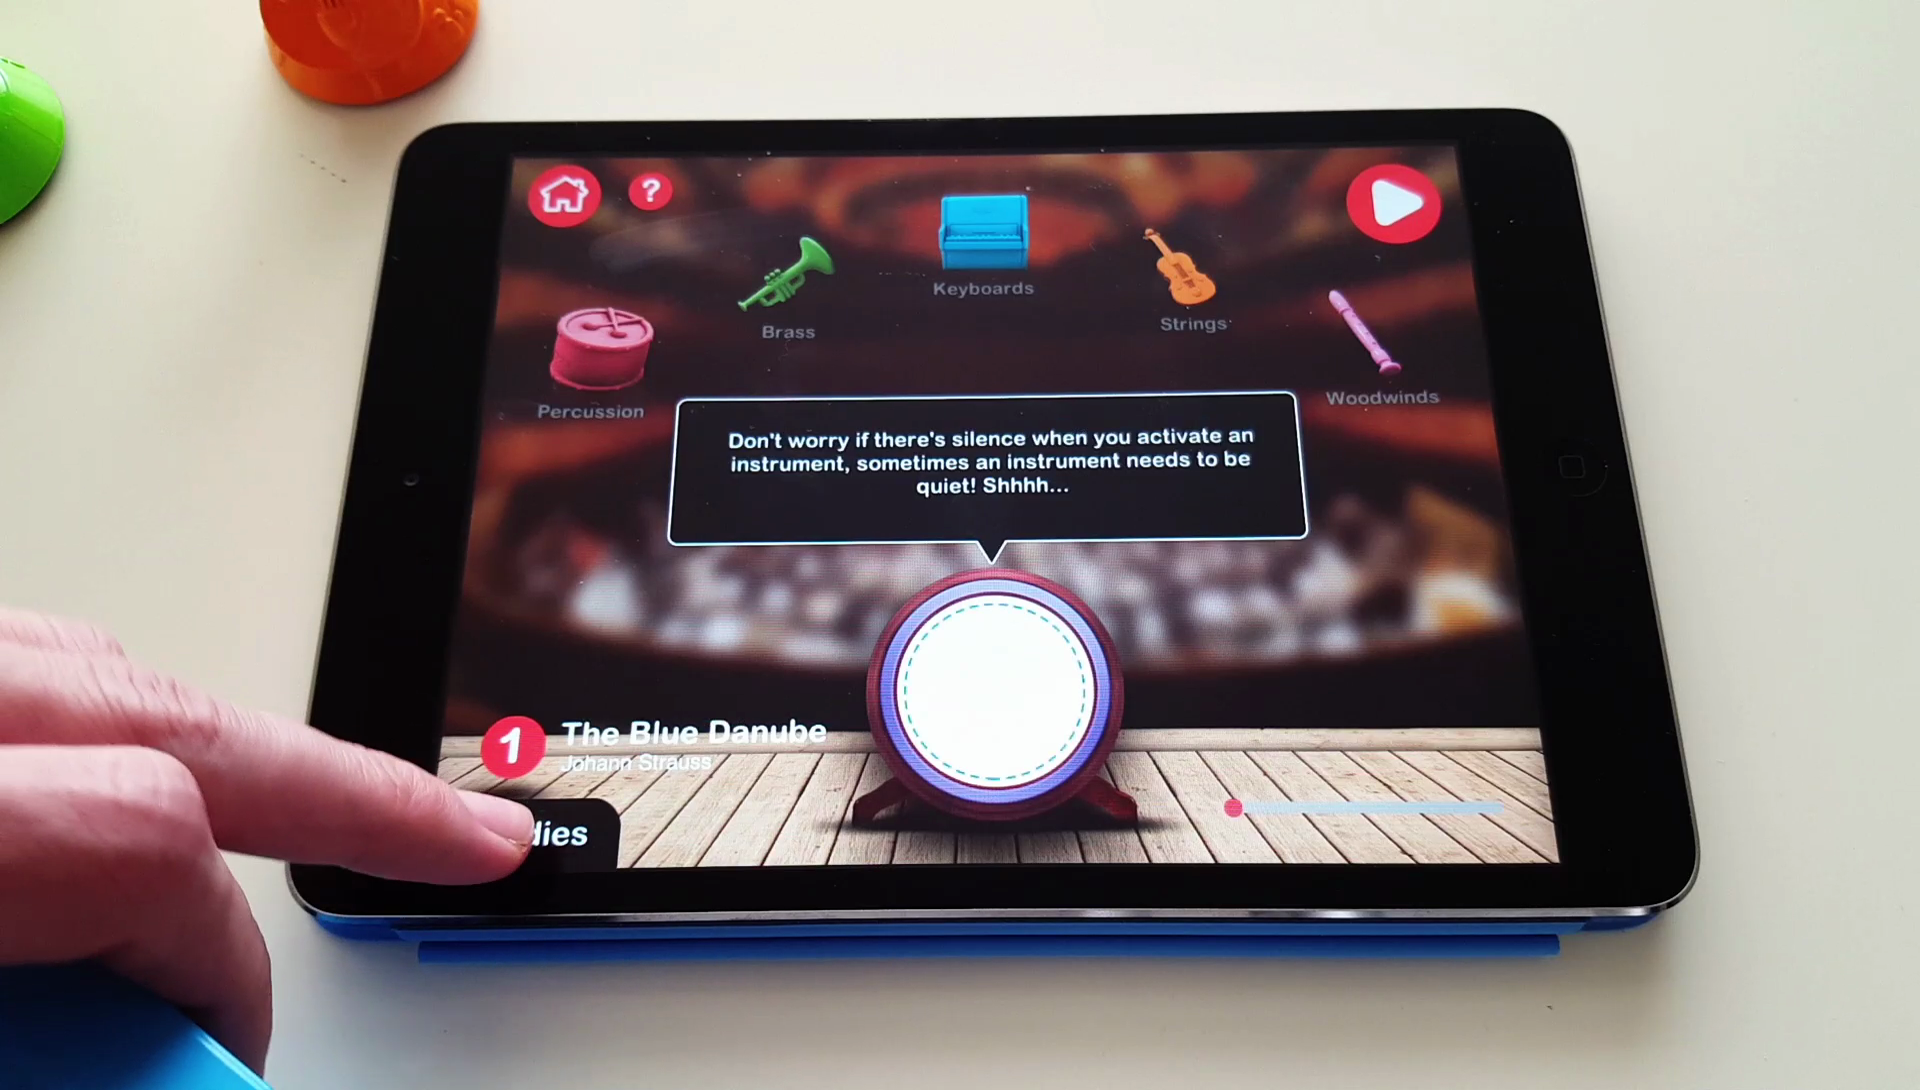
\includegraphics[width=350pt]{graphics/game-play/choose_melody_conducting.png}
  \vspace{0.05cm}
  \caption{Opening melodies menu in playing game mode}
\end{figure}

\begin{figure}[ht!]
  \centering
  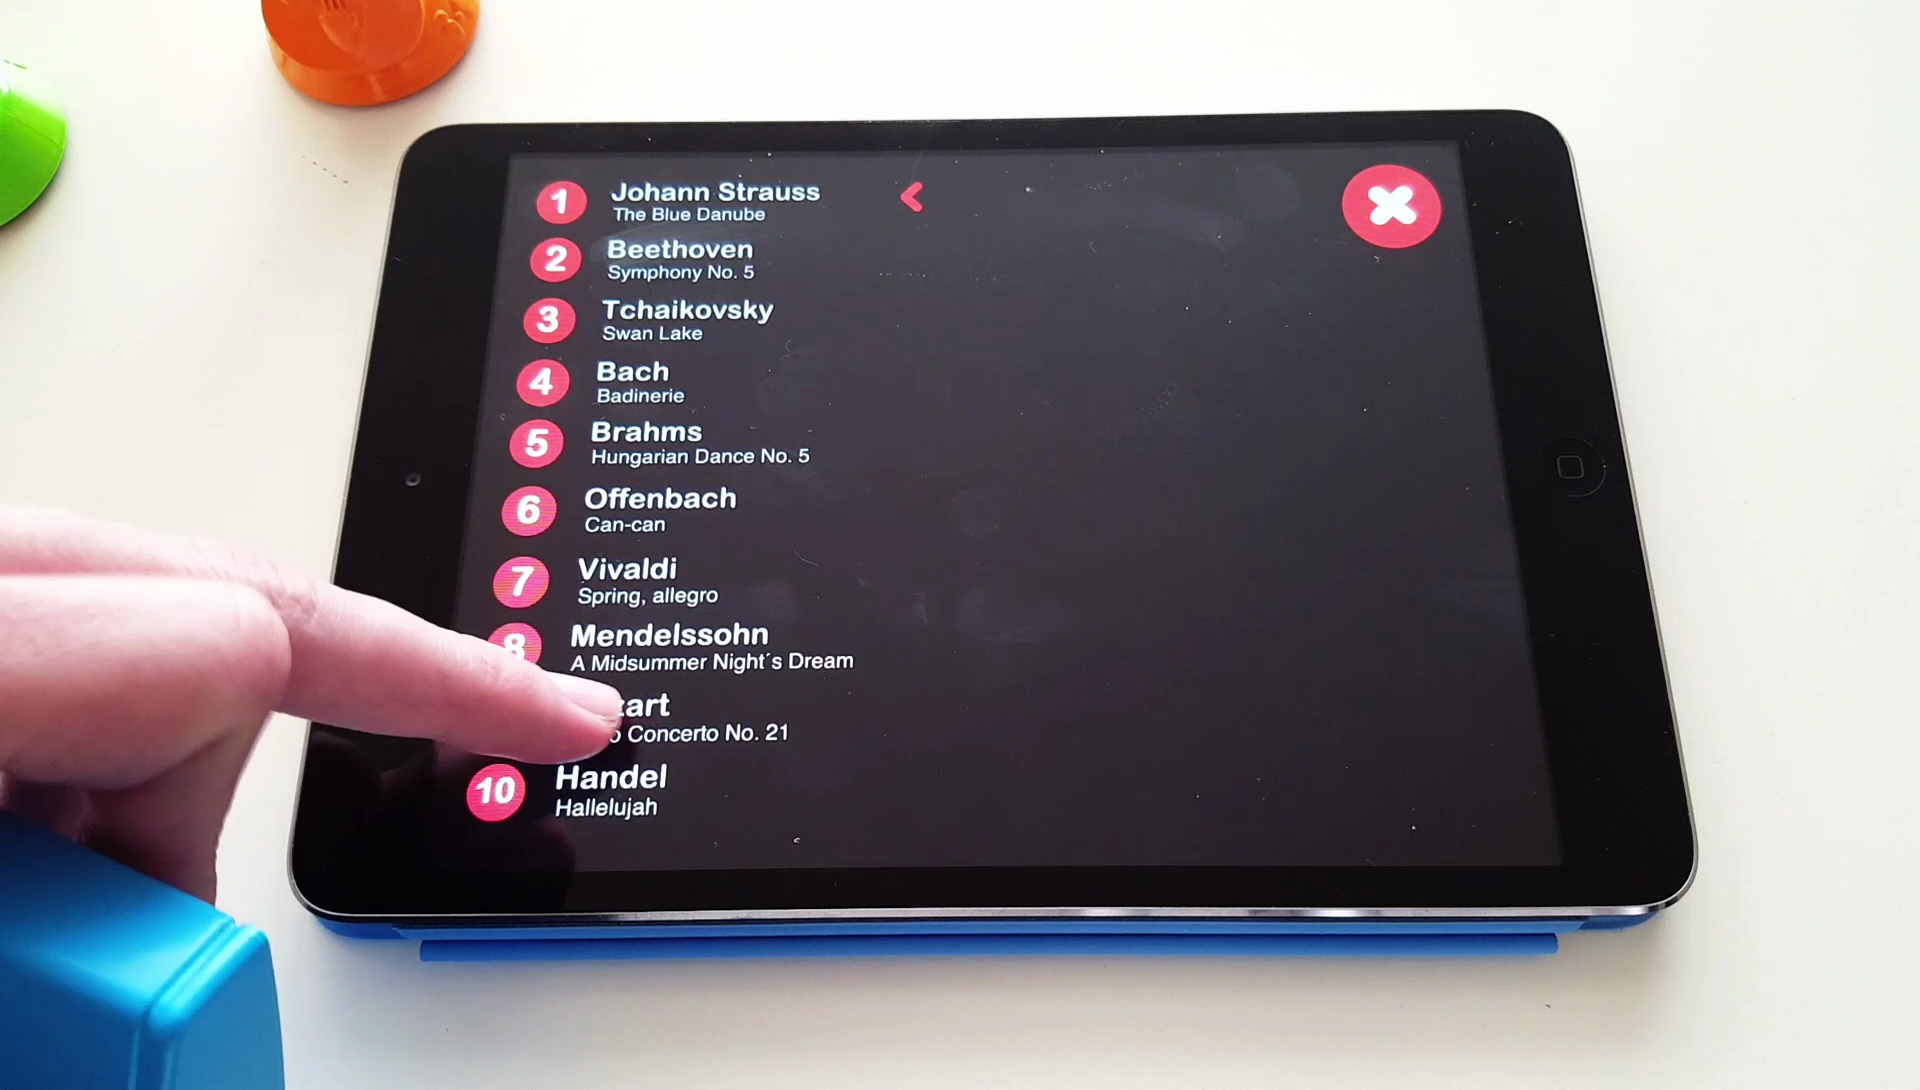
\includegraphics[width=350pt]{graphics/game-play/change_melody_conducting.png}
  \vspace{0.05cm}
  \caption{Changing melody to be played in playing game mode}
  \vspace{1cm}

  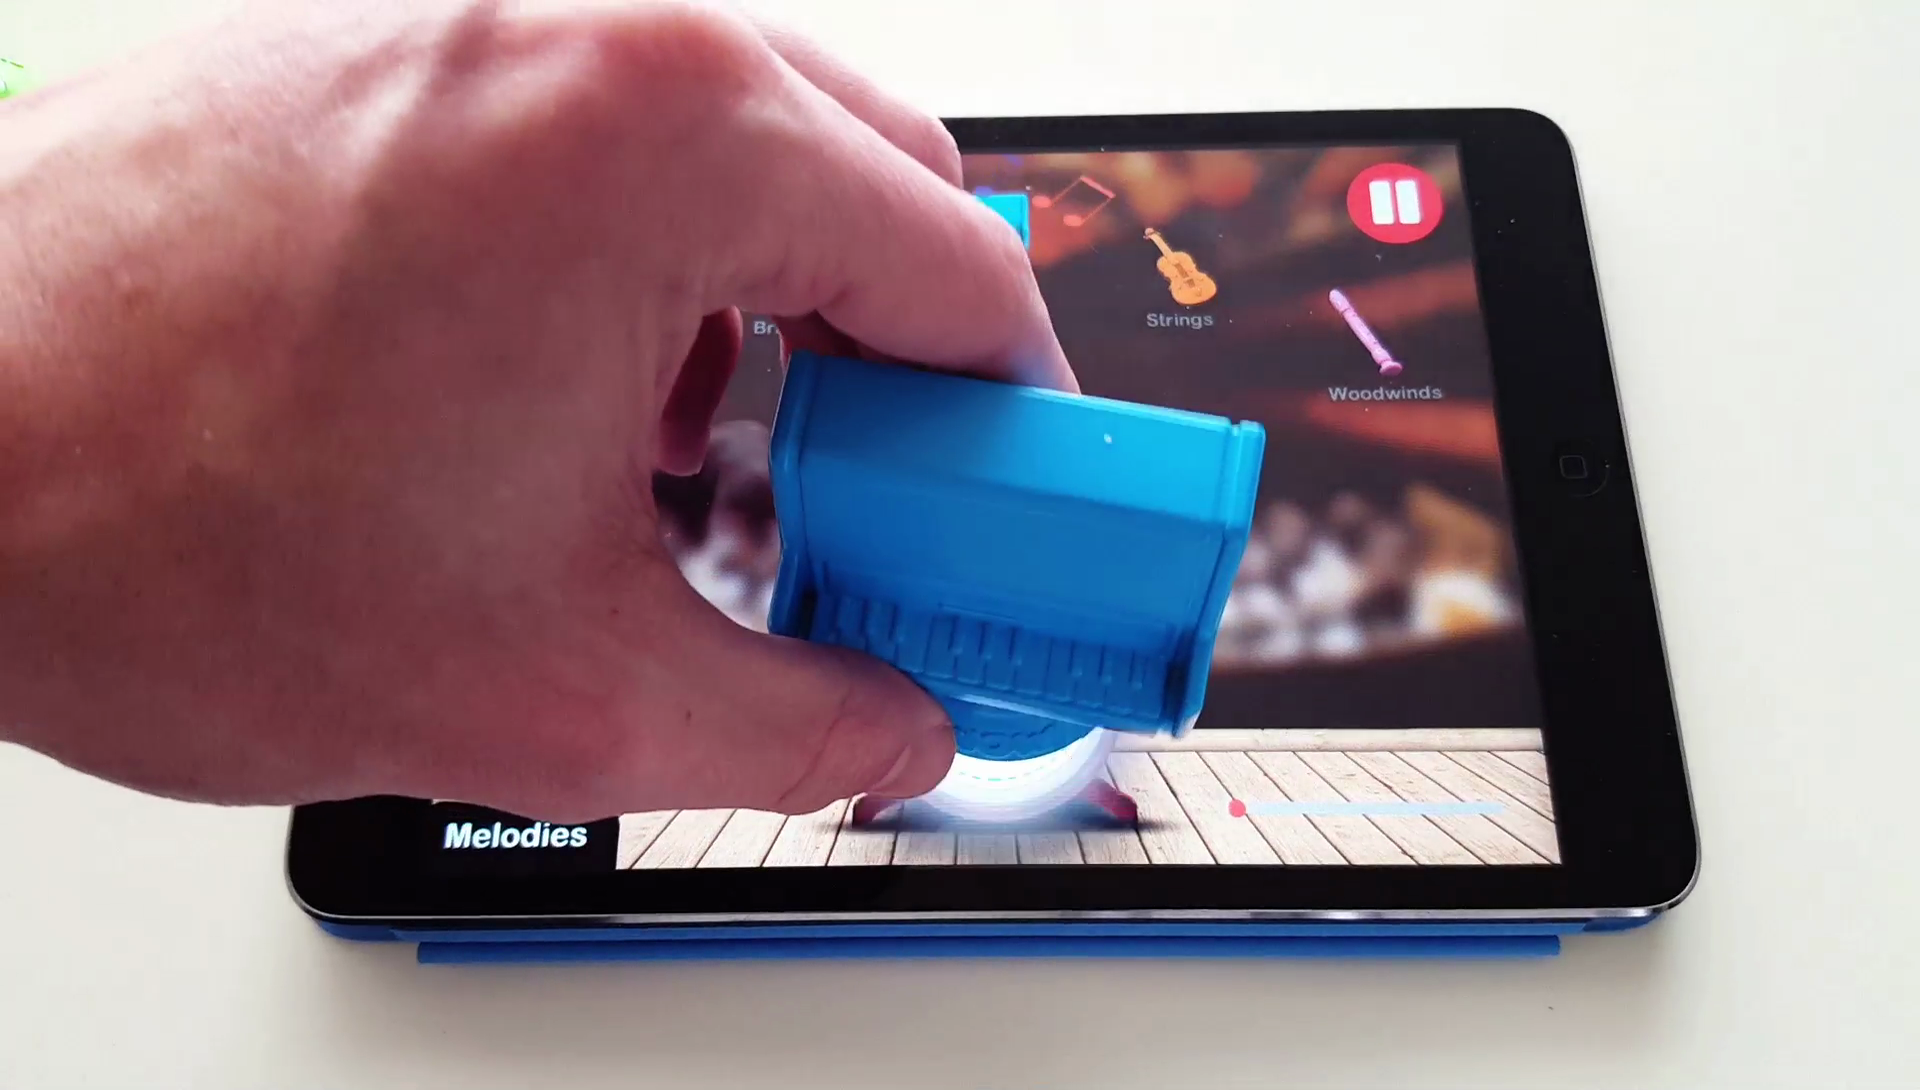
\includegraphics[width=350pt]{graphics/game-play/activate_keyboards_family.png}
  \vspace{0.05cm}
  \caption{Activating keyboards family}
\end{figure}

\begin{figure}[ht!]
  \centering
  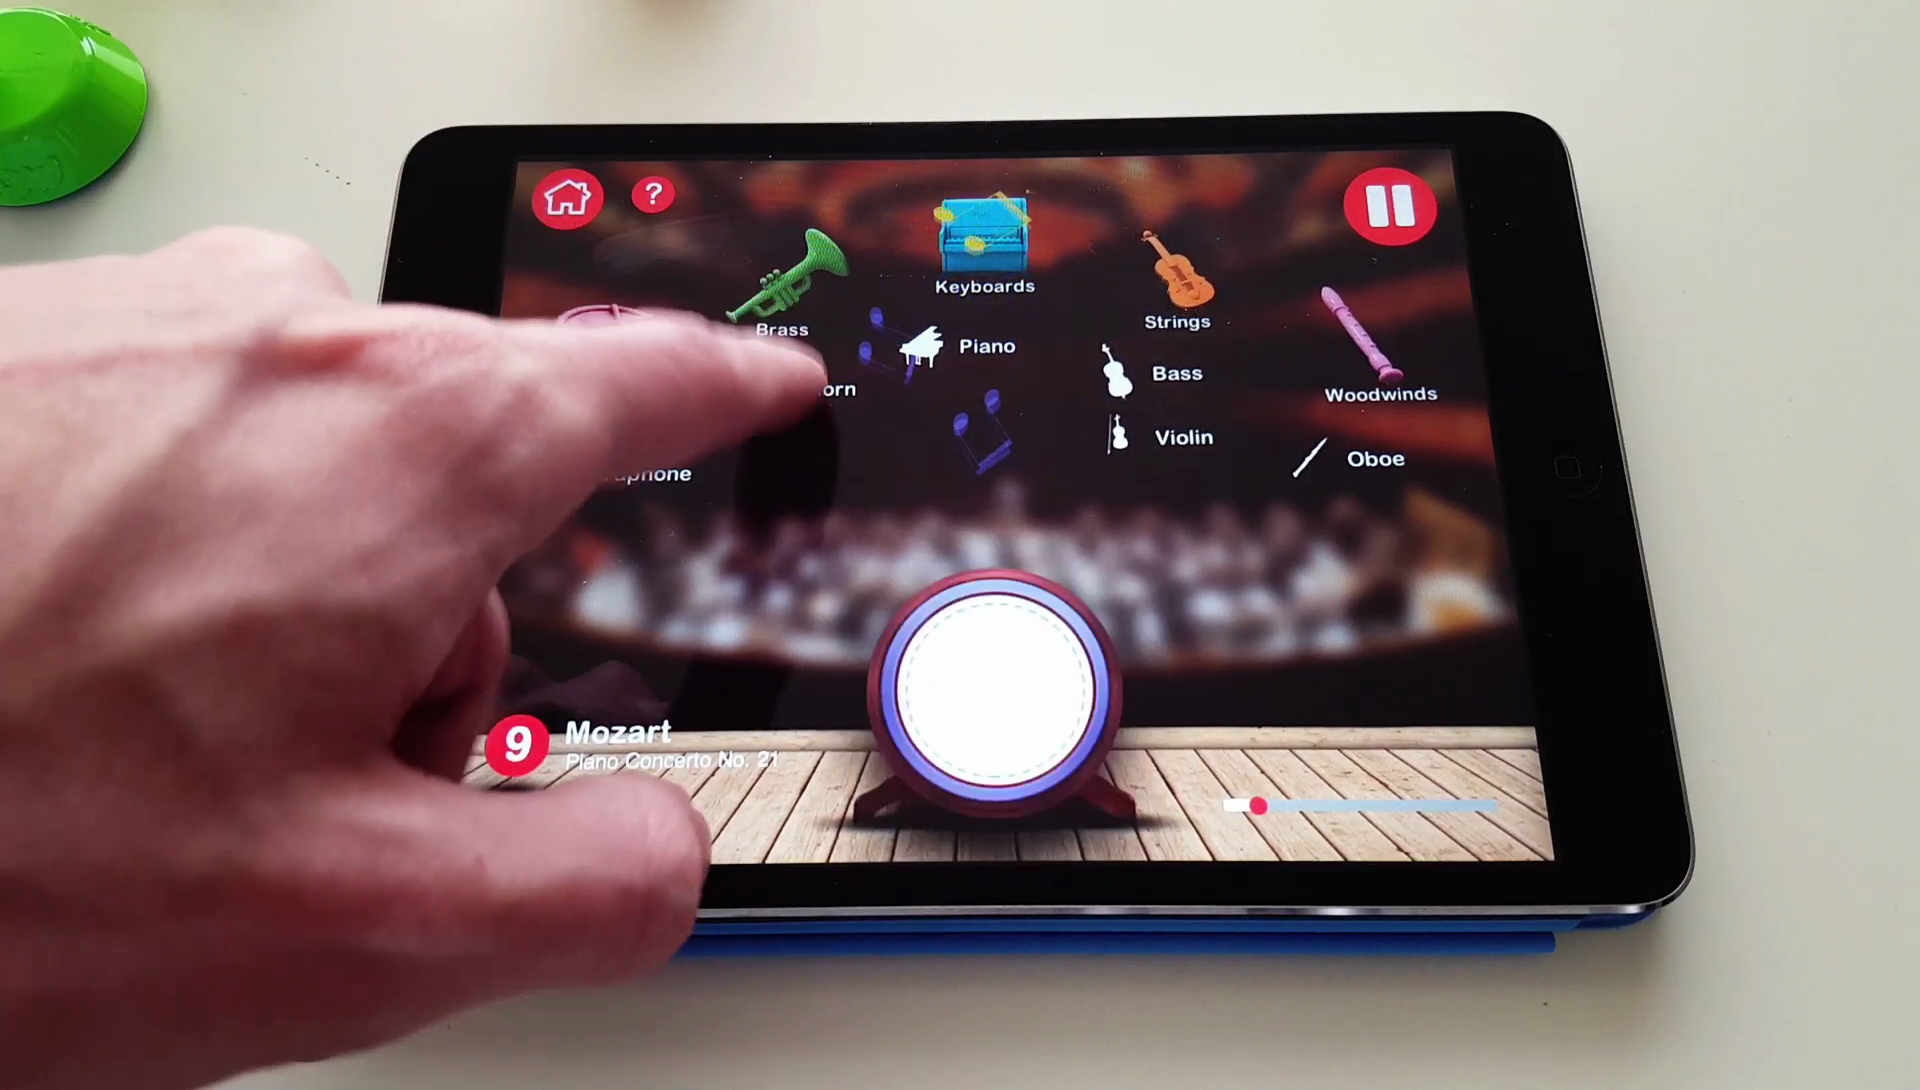
\includegraphics[width=350pt]{graphics/game-play/disable_instrument_conducting.png}
  \vspace{0.05cm}
  \caption{Disabling instrument}
  \vspace{1cm}

  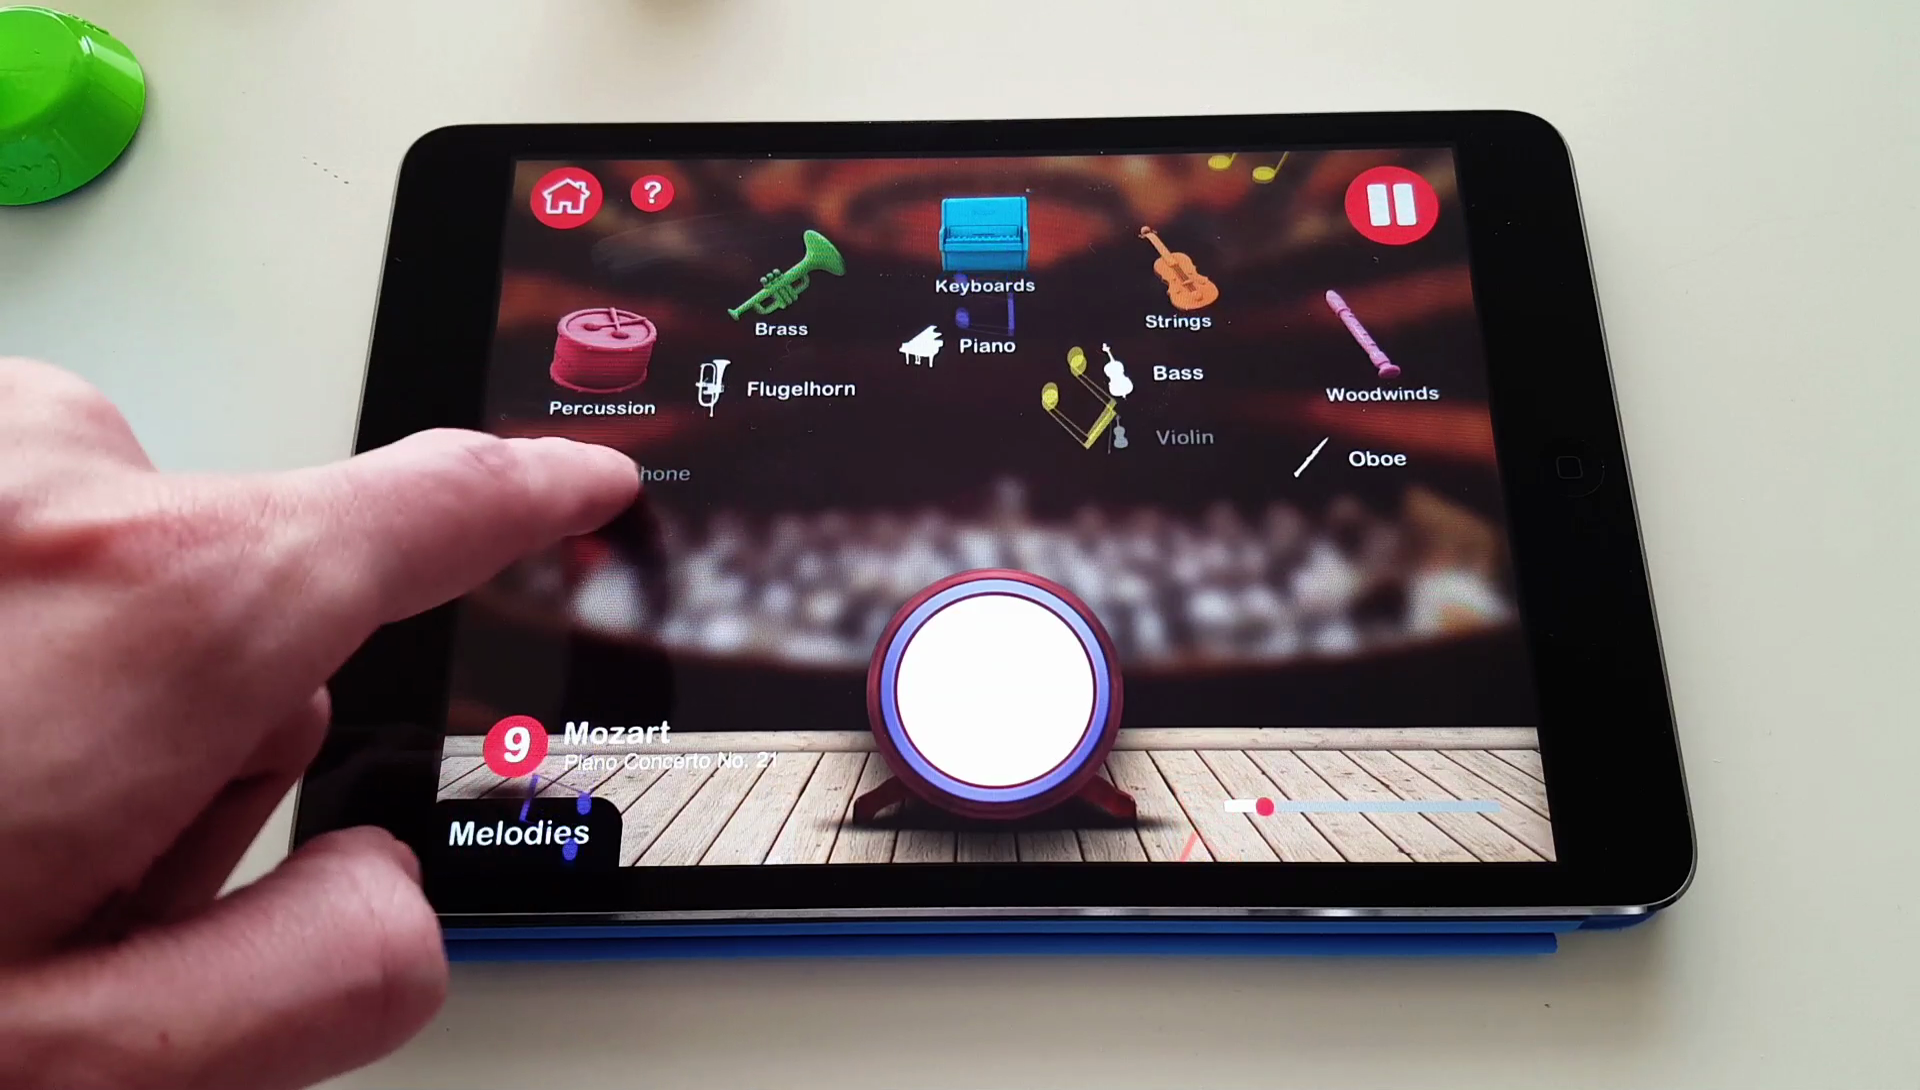
\includegraphics[width=350pt]{graphics/game-play/enable_instrument_conducting.png}
  \vspace{0.05cm}
  \caption{Enabling instrument}
\end{figure}

\section{Discovering game mode}

\begin{figure}[ht!]
  \centering
  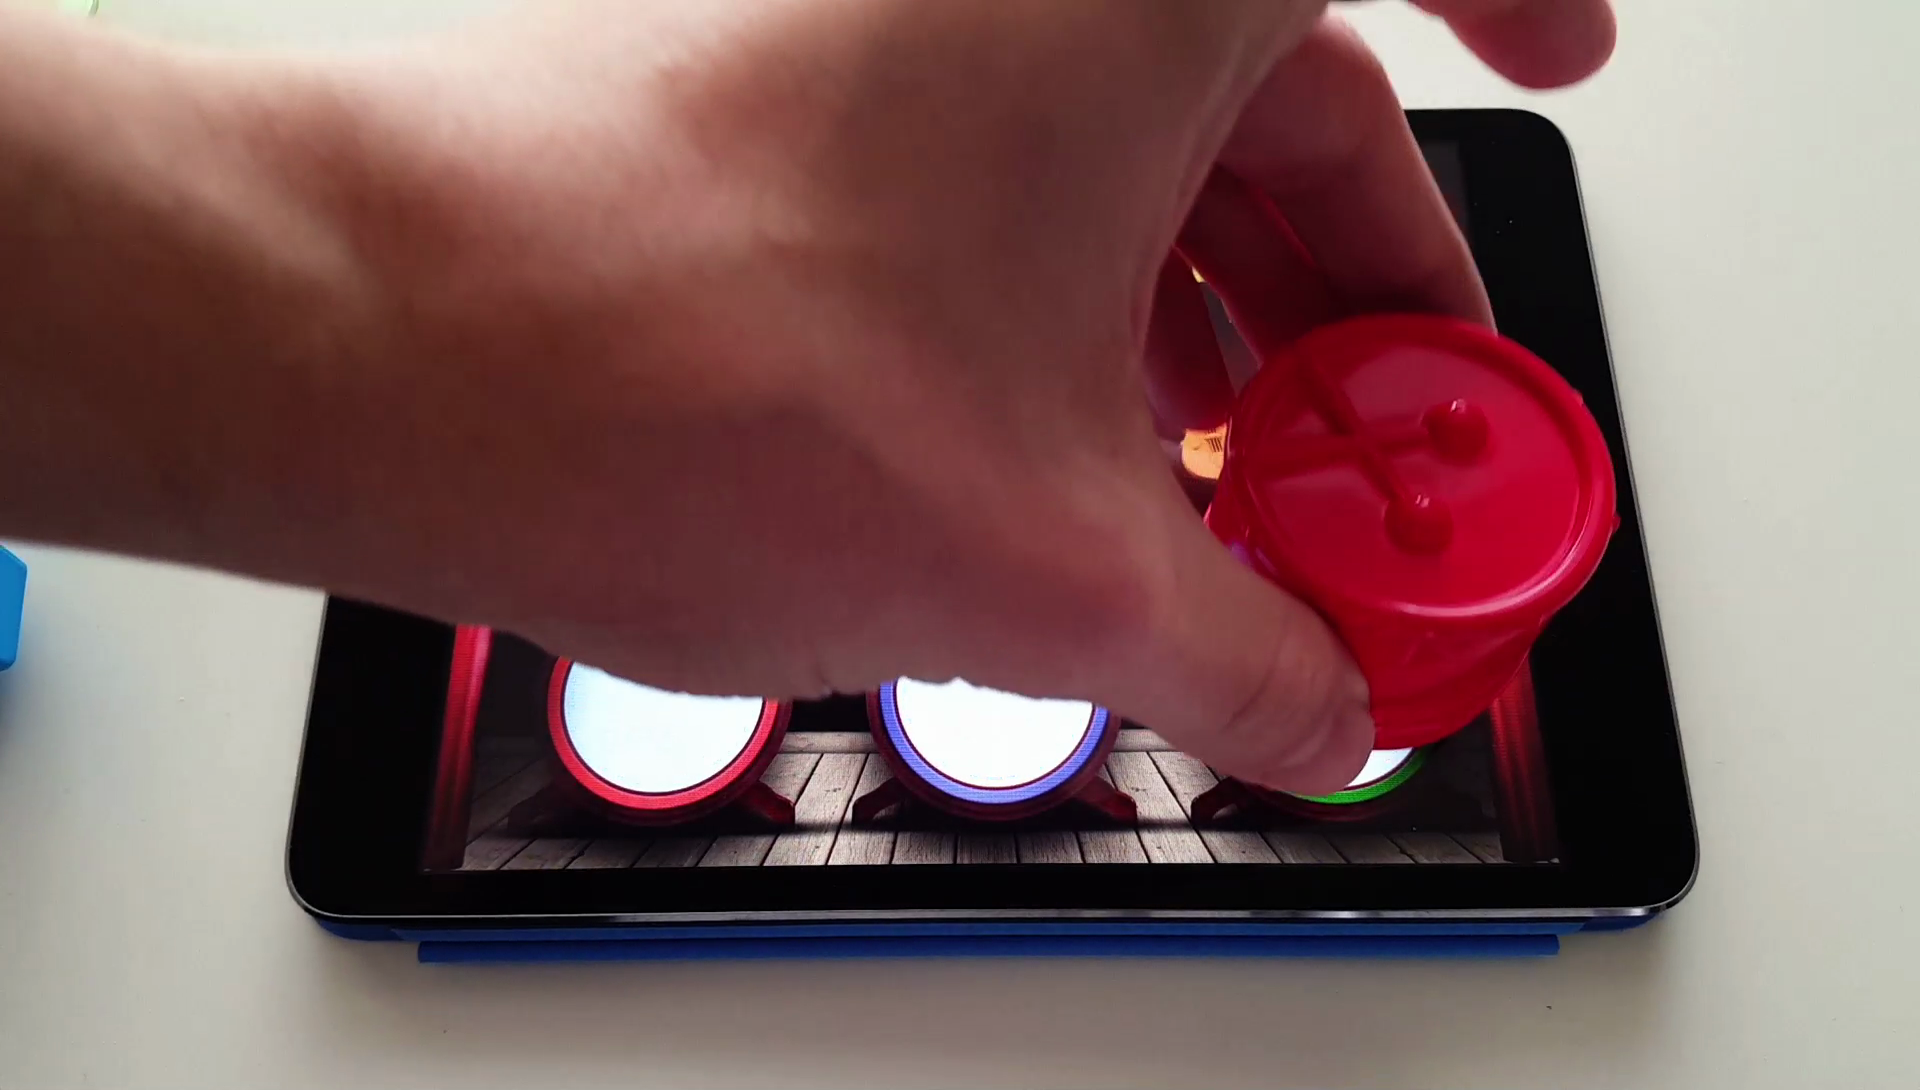
\includegraphics[width=350pt]{graphics/game-play/enter_discovering_mode.png}
  \vspace{0.05cm}
  \caption{Entering discovering game mode from home screen}
  \vspace{1cm}

  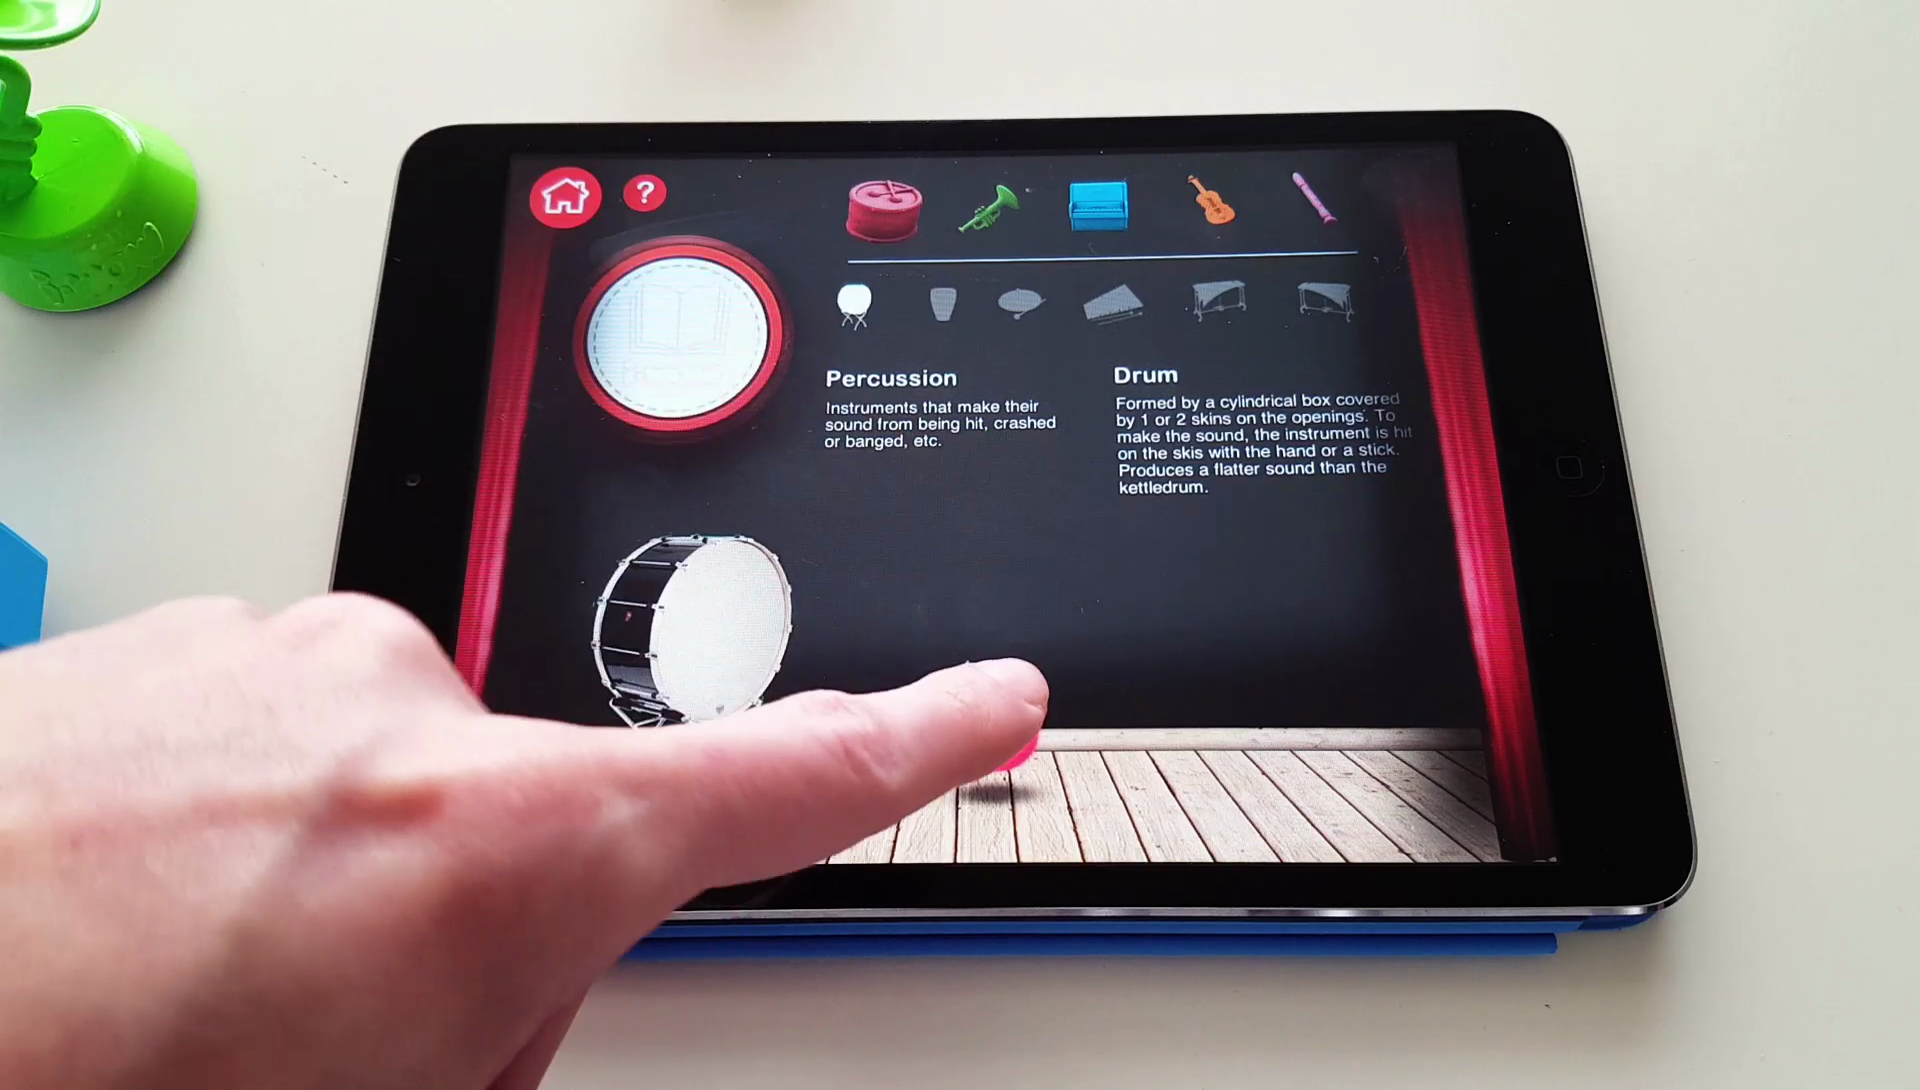
\includegraphics[width=350pt]{graphics/game-play/instrument_sound_discovering.png}
  \vspace{0.05cm}
  \caption{Playing instrument sound}
\end{figure}

\begin{figure}[ht!]
  \centering
  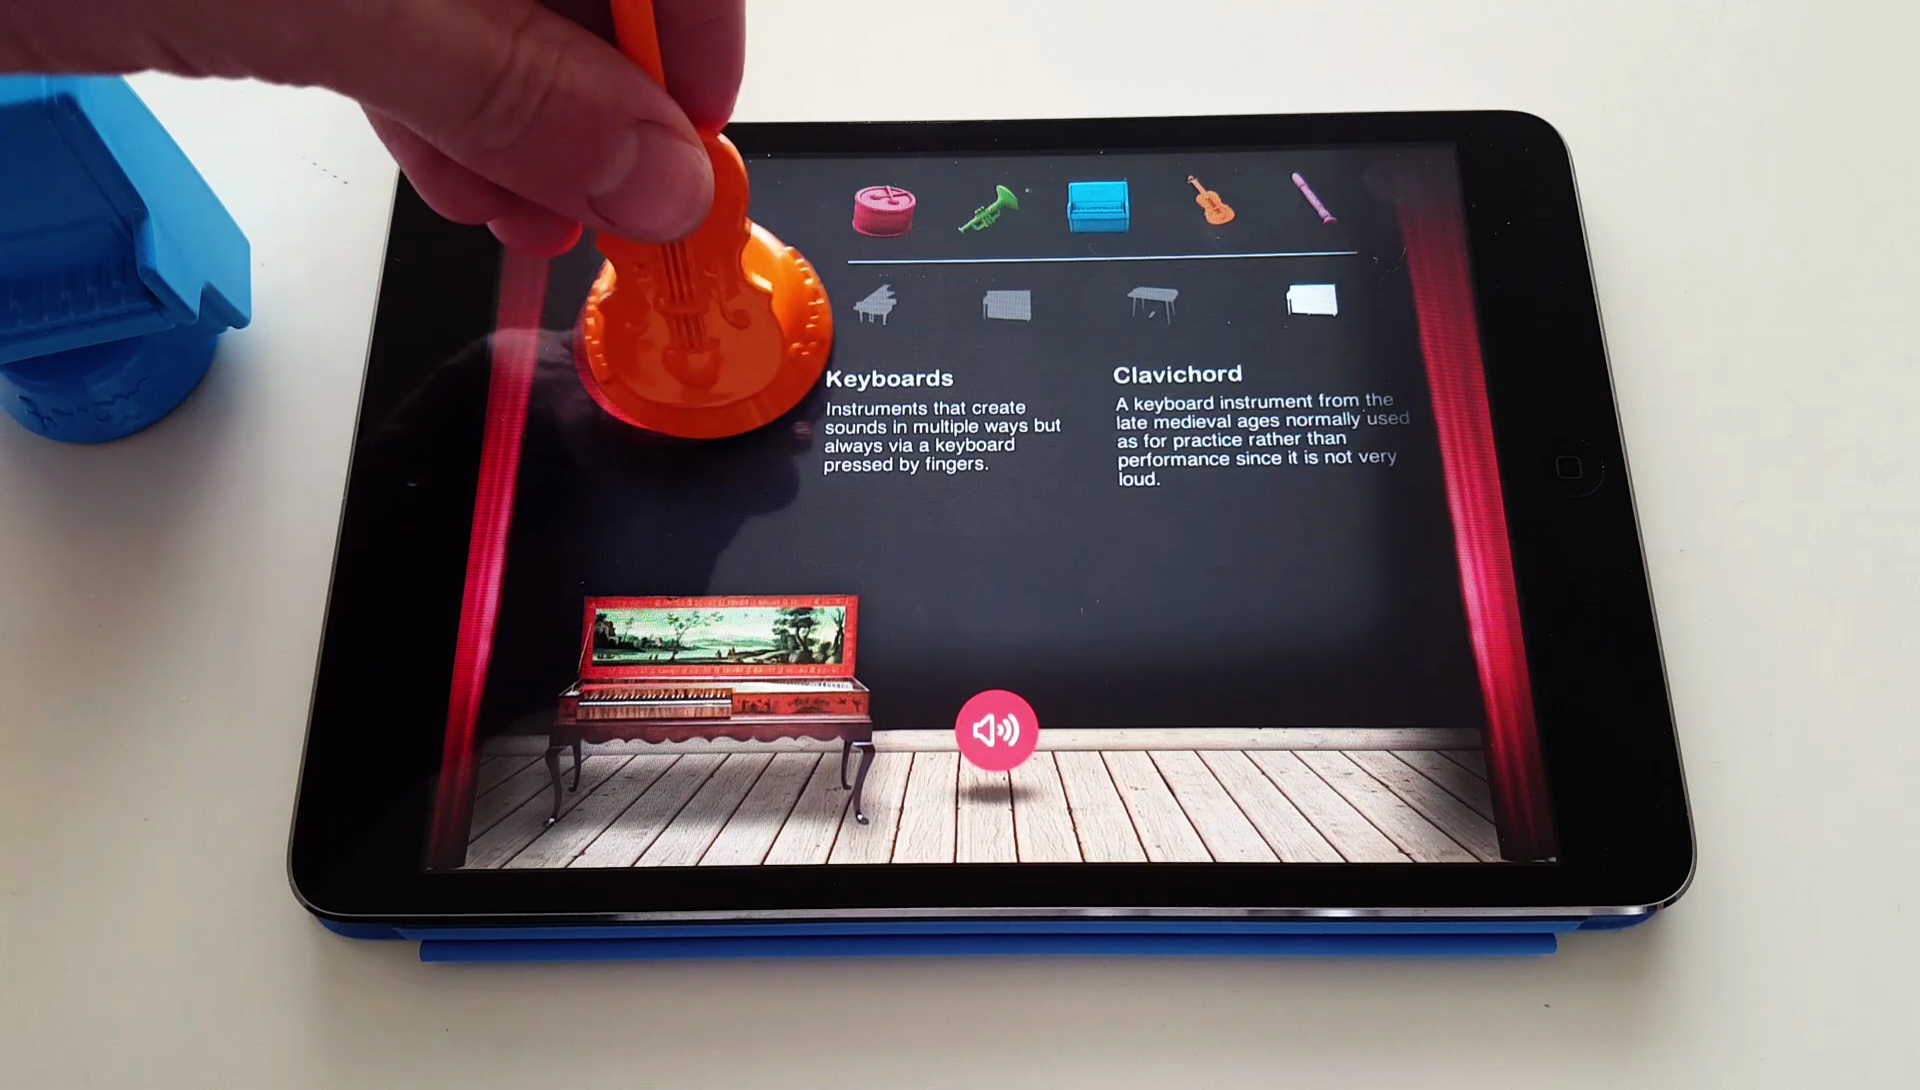
\includegraphics[width=350pt]{graphics/game-play/change_family_discovering.png}
  \vspace{0.05cm}
  \caption{Changing family in discovering game mode}
  \vspace{1cm}

  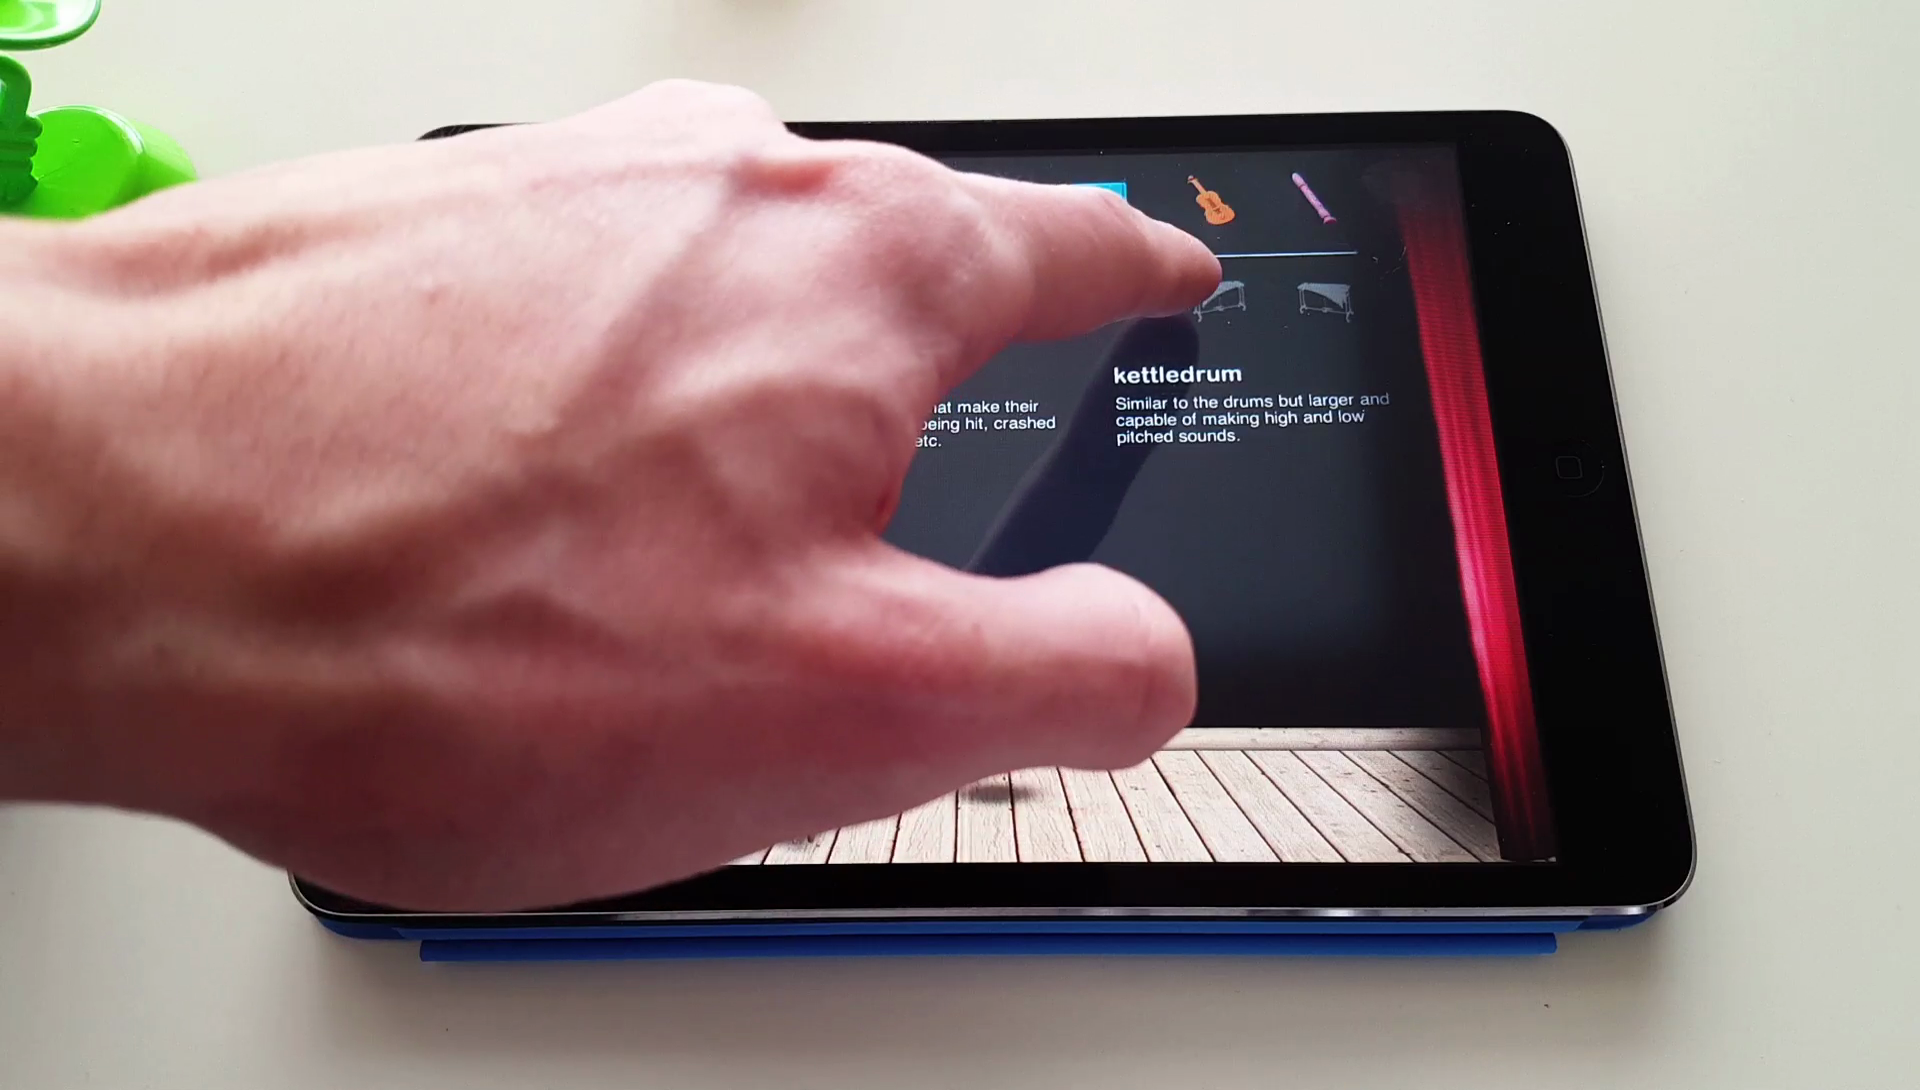
\includegraphics[width=350pt]{graphics/game-play/change_instrument_discovering.png}
  \vspace{0.05cm}
  \caption{Changing instrument in discovering game mode}
\end{figure}

